%\documentclass[12pt, a4paper, oneside]{book}
\documentclass[12pt, a4paper, titlepage, twoside]{book}
%\documentclass[a4paper,11pt,twoside]{report}
% TODO: should I change it to report? what is twoside?
\usepackage[latin1]{inputenc}
\usepackage[cyr]{aeguill}

% farzaneh \usepackage[francais]{babel}
%\usepackage{afterpage}
\usepackage{fancyhdr, ifpdf}
\usepackage{array}
\usepackage{multirow}
\usepackage[latin1]{inputenc}
\usepackage[titletoc]{appendix}
%\def\pgfsysdriver{pgfsys-dvipdfm.def}
%\usepackage{tikz}

\usepackage{textcomp}

\usepackage{verbatim} 

\usepackage{listings}
\usepackage{hyperref}
\usepackage[table]{xcolor}% http://ctan.org/pkg/xcolor
\usepackage{hhline}
\usepackage{framed}
\usepackage{pifont}% http://ctan.org/pkg/pifont
\usepackage{tikz}
\usepackage{float}
\def\checkmark{\tikz\fill[scale=0.4](0,.35) -- (.25,0) -- (1,.7) -- (.25,.15) -- cycle;} 
\newcommand{\cmark}{\ding{51}}%
\newcommand{\xmark}{\ding{55}}%
\usepackage{algorithm}
\usepackage{algorithmic}
%\usepackage{amsmath}
%\usepackage{algorithm}
%\usepackage[noend]{algpseudocode}
\usepackage{setspace}
\usepackage{perpage} %the perpage package
\MakePerPage{footnote} %the perpage package command

% Uncomment to show frames
%\usepackage{showframe}

%\setlength{\hoffset}{0.5cm}
\setlength{\oddsidemargin}{1.3cm}
\setlength{\evensidemargin}{0.8cm}

%\setlength{\marginparwidth}{2cm}
  
%Pour montrer les label
%\usepackage{showkeys}
%\usepackage{showlabels}

%\usepackage{varioref}
%\usepackage[french]{varioref} 
\usepackage{booktabs}
\newcommand{\otoprule}{\midrule[\heavyrulewidth]}

\usepackage{amsmath,amssymb,amstext,mathtext}

\definecolor{LightBlue}{rgb}{0.8,0.8,1.0}
% Uncomment one of these line depending whether you want to see the draft or the final version.
%\usepackage[draft]{graphicx}
% TODO: What is a draft?
\usepackage{graphicx}
\graphicspath{{./figures/}{./logo/}}

\makeatletter
\def\cleardoublepage{\clearpage\if@twoside \ifodd\c@page\else
\hbox{}
\vspace*{\fill}
\begin{center}
\end{center}
\vspace{\fill}
\thispagestyle{empty}
\newpage
\if@twocolumn\hbox{}\newpage\fi\fi\fi}
\makeatother

\pagestyle{fancyplain}

% some redefination of the headers and footers
\renewcommand{\chaptermark}[1]%
                 {\markboth{#1}{}}
\renewcommand{\sectionmark}[1]%
                 {\markright{\thesection\ #1}}
\lhead[\fancyplain{}{\thepage}]%
      {\fancyplain{}{\rightmark}}
\rhead[\fancyplain{}{\leftmark}]%
      {\fancyplain{}{\thepage}}
\cfoot{}
\sloppy

% Farzaneh \ifpdf
% Farzaneh   \usepackage[pdftex]{graphicx}
% TODO: do I need this?
%   \pdfinfo {
%      /Title (A monolithic microrobotic arm in silicon)
 %     /Subject (Rapport de projet de semestre)
 %     /Author (Marc Stranczl)
 %     /Keywords (SOI)
 %  }
% Farzaneh \else
% Farzaneh   \usepackage{graphicx}
% Farzaneh \fi



\begin{document}


%% http://en.wikibooks.org/wiki/LaTeX/Title_Creation
% Adjusted for EPFL template


\begin{titlepage}

\begin{center}

\raisebox{2cm}[-2cm][-2cm]{
\hspace{-1.5cm}

  \footnotesize
  \begin{tabular}{@{\hspace{10pt}}l@{\hspace{0pt}} l@{\hspace{10pt}}}
  %  \cline{0-0}     &\multirow{5}{*}{\hspace{10pt}\raisebox{-1ex}{
\includegraphics[width=0.4\columnwidth]{CERN-logo}}}\\
    \multirow{5}{*}{\hspace{10pt}\raisebox{-1ex}{
\includegraphics[height=0.2\textheight]{CERN-logo}}}    & \multirow{5}{*}{\hspace{10pt}\raisebox{-1ex}{
\includegraphics[width=0.4\columnwidth]{EPFL_LOG_QUADRI_Red}}}\\

         \\
    \\
    \raisebox{1.2ex}{INSTITUT DE MICROTECHNIQUE | Laboratoire de Microsyst�mes} \\
    %\scriptsize CH -- 1015 LAUSANNE \\

  \end{tabular}%
}

\vspace{1\baselineskip}
\Huge

\newcommand{\HRule}{\rule{\linewidth}{0.3mm}}


    {\huge \bfseries  A monolithic microrobotic arm \\ in silicon} \\
    {\Large \bfseries  Microrobot monolithique en silicium} \\
	\vspace{3mm}    
    \textsc{\Large Projet de Semestre} \Large (Automne 2009) \\
    \Large Section Microtechnique
    
    %\HRule \\[0.2cm]
	
	\vspace{3mm}
	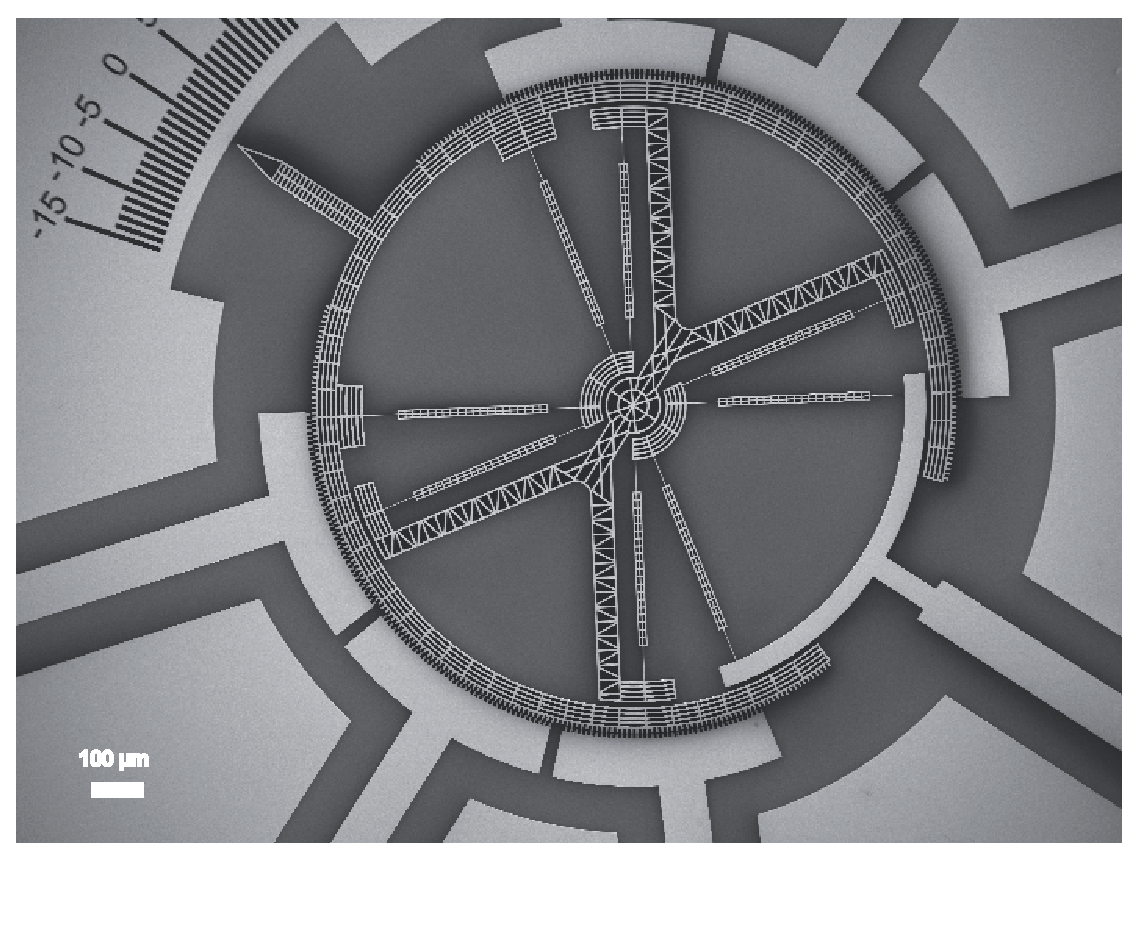
\includegraphics[height=6 cm]{fig_couverture}
	\vspace{3mm}
	\HRule 
	
	\emph{Auteur:} \\
	Marc \textsc{Stranczl}\\
    \vspace{0.5cm}
    \emph{Sous la supervision de:} \\   

    Prof. Martinus \textsc{Gijs}, LMIS2 \\   
    Dr. Christophe \textsc{Yamahata}, LMIS 2\\

	\vspace{0.5cm}
    % Bottom of the page
    \emph{Remis le: 8 janvier 2010}
	%{\large \today}


\end{center}


\end{titlepage}

\newpage
\thispagestyle{empty}
\mbox{}
%\maketitle

%\begin{titlepage}
%\fancyhf{}

% http://en.wikibooks.org/wiki/LaTeX/Title_Creation
% Adjusted for EPFL template


\begin{titlepage}

\begin{center}

\raisebox{2cm}[-2cm][-2cm]{
\hspace{-1.5cm}

  \footnotesize
  \begin{tabular}{@{\hspace{10pt}}l@{\hspace{0pt}} l@{\hspace{10pt}}}
  %  \cline{0-0}     &\multirow{5}{*}{\hspace{10pt}\raisebox{-1ex}{
\includegraphics[width=0.4\columnwidth]{CERN-logo}}}\\
    \multirow{5}{*}{\hspace{10pt}\raisebox{-1ex}{
\includegraphics[height=0.2\textheight]{CERN-logo}}}    & \multirow{5}{*}{\hspace{10pt}\raisebox{-1ex}{
\includegraphics[width=0.4\columnwidth]{EPFL_LOG_QUADRI_Red}}}\\

         \\
    \\
    \raisebox{1.2ex}{INSTITUT DE MICROTECHNIQUE | Laboratoire de Microsyst�mes} \\
    %\scriptsize CH -- 1015 LAUSANNE \\

  \end{tabular}%
}

\vspace{1\baselineskip}
\Huge

\newcommand{\HRule}{\rule{\linewidth}{0.3mm}}


    {\huge \bfseries  A monolithic microrobotic arm \\ in silicon} \\
    {\Large \bfseries  Microrobot monolithique en silicium} \\
	\vspace{3mm}    
    \textsc{\Large Projet de Semestre} \Large (Automne 2009) \\
    \Large Section Microtechnique
    
    %\HRule \\[0.2cm]
	
	\vspace{3mm}
	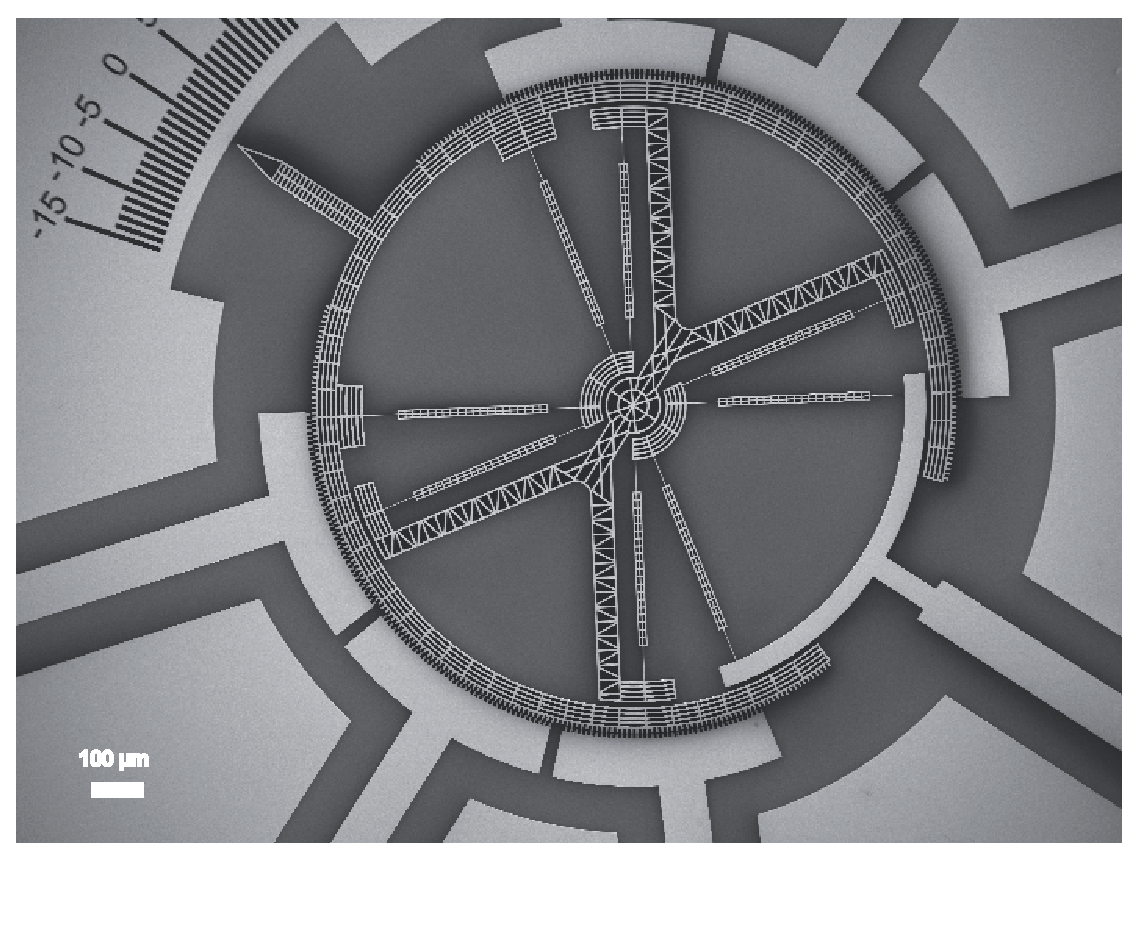
\includegraphics[height=6 cm]{fig_couverture}
	\vspace{3mm}
	\HRule 
	
	\emph{Auteur:} \\
	Marc \textsc{Stranczl}\\
    \vspace{0.5cm}
    \emph{Sous la supervision de:} \\   

    Prof. Martinus \textsc{Gijs}, LMIS2 \\   
    Dr. Christophe \textsc{Yamahata}, LMIS 2\\

	\vspace{0.5cm}
    % Bottom of the page
    \emph{Remis le: 8 janvier 2010}
	%{\large \today}


\end{center}


\end{titlepage}

\newpage
\thispagestyle{empty}
\mbox{}

%\end{titlepage}

\chapter*{Acknowledgements}
\thispagestyle{empty}
I would like to use this opportunity to express my special appreciation and thanks to Mr. Sebastian Lopienski for his aspiring guidance and illuminating views on a number of issues related to the project. I would also like to express my gratitude to Professor Philippe Janson for his invaluable advice on the progress of the project and the quality of this thesis, and Dr. Stefan Lueders for his continuous support and help with writing this thesis. In addition, a big thank you to my family and friends for their motivating words and their endless love. I would like to dedicate my work to my sister, Atefeh, without whose love and support, it would have been impossible for me to pursue a master degree at EPFL. 
\clearpage
\chapter*{Abstract}
\thispagestyle{empty}

It is crucial for big organizations like CERN with a very large web landscape to ensure the security of their web resources. One can use various open source or commercial web scanners to scan websites and look for common, well-known web vulnerabilities. However, these scanners usually fail to find vulnerabilities that are discovered every day in software products and commonly used libraries. The main objective of this project is to automate the procedure for detecting vulnerable web applications remotely and when new vulnerabilities emerge. For this purpose, we will introduce a tool that monitors vulnerability sources to find newly discovered vulnerabilities, and detects CERN resources that use vulnerable third party products. In addition, we introduce another tool that facilitates scanning CERN resources for critical vulnerabilities in emergency cases, specially when a vulnerability is not specific to a certain, detectable third party product.
%% start the show...
% TODO: I'd rather start it after the table

\pagenumbering{roman}
\setcounter{page}{1}
\pagenumbering{arabic}

\tableofcontents

%\listoffigures
%\listoftables



\chapter{Introduction}
\label{introduction}
\thispagestyle{empty}
Over the past decade, web applications have been embraced by many companies to deliver their main services to customers. One can think of different reasons for this increase in popularity: ubiquity of web browsers makes it convenient to use them as a client; web applications can be updated and maintained locally with no need to distribute or install software on the client side and web applications are cross-platform compatible.
Another reason for the increasing popularity of web applications is the simplicity of developing them. Nowadays there are many web application frameworks and content management systems that facilitate rapid application development. This simplicity comes with a cost: securing a web application is difficult. Web applications include code that resides on the web servers, application servers, databases, and back-end systems of an organization. The potential for a security breech exists in each of these layers. This opens the door to attackers trying to manipulate the application logic to perpetrate their misdeeds\cite{secure_web}. In this project, we are going to focus on approaches for maintaining the security of web applications at CERN\footnote{European organization for nuclear research}. CERN is a large particle physics research organization and it manages thousands of websites and web servers for different purposes. Ensuring the security of this large web landscape is one of the main priorities of its Computer Security Team.

\paragraph{}
Even if a web application is designed to be as secure as possible, vulnerabilities will invariably be discovered over time in its code or in the code of underlying packages it uses and relies on. Therefore, to continue ensuring that the application remains secure, it is important to constantly check for newly discovered vulnerabilities and make sure that the application is not affected. This task is easier for the application designers themselves, who are aware of all the technologies that are used in their application; however, in many organizations like CERN, any employee can set up a web server or launch a website and few employees bother to monitor their own web applications for security vulnerabilities. It is the job of the Computer Security Team to scan these various web servers and websites and detect all vulnerabilities remotely.
\paragraph{}
There are two main approaches for ensuring the security of web applications: The first approach is to use the available automatic scanning tools, such as Acunetix or Skipfish\footnote{Google open source security reconnaissance tool}, to detect vulnerabilities. Using this approach, we can find common vulnerabilities, but when a new vulnerability emerges we have to wait for the new version of the scanning tool to be released and include tests for the new vulnerability. Also, due to the complexity of these tools, it is a time consuming task to configure them for a specific scanning purpose. 
\paragraph{}
The second approach is to keep an eye on vulnerability sources, databases, security mailing lists, etc. to get informed about new vulnerabilities as soon as possible. This way we will not miss any critical vulnerabilities. The next step is to use the vulnerability information to detect any vulnerable resources in the organization. 
\section{Project Focus}
The focus of this project is going to be on the second approach, meaning that we are going to propose two new methods of identifying vulnerable resources affected by newly disclosed vulnerabilities or vulnerabilities that common web scanners fail to identify. 
\paragraph{}
The disclosed vulnerabilities regularly appear on different sources, such as mailing lists, databases, forums, etc. These vulnerabilities might be disclosed with a list of affected products, for example; a vulnerability that affects all websites using Drupal Content Management Systems. In Chapter \ref{vulnerability-notification-tool}, we take advantage of publicly available vulnerability sources and describe a tool we developed --Vulnerability Notification Tool-- that first reports all newly disclosed vulnerabilities and in a second step delivers lists of vulnerable components (from vulnerability information) and uses those lists to alert the CERN Computer Security Team about web applications that may be vulnerable as a result of using those components.
\paragraph{}
On the other hand, sometimes the vulnerabilities are not specific to a certain product, e.g. a vulnerability found in a network protocol or an encryption algorithm, or it is impossible with current tools to detect if a resource is using a certain product. Chapter \ref{scanner} introduces a complementary new tool we developed --Scanner-- that facilitates scanning CERN web applications components with simple (home-grown) security tests to detect individual vulnerabilities on potentially affected components. Heartbleed\footnote{Critical OpenSSL vulnerability, discovered in April 2014} is a good example of a case when it was critical to detect vulnerable resources as soon as possible. The vulnerability was not specific to a single detectable product and most organizations had to use their own (or publicly available) scripts to detect the vulnerability and patch the resources.

\section{Vulnerability Definition}
According to the MITRE CVE initiative\footnote{\url{http://cve.mitre.org/about/terminology.html\#Dist}}, a vulnerability is a mistake in software that can be directly used by a hacker to gain access to a system or network. A vulnerability would allow an attacker to:
\begin{itemize}
\item execute unauthorized commands
\item access data that is contrary to the specified access restrictions for that data
\item pose as another entity or user
\item conduct a denial of service
\end{itemize}

Note that a vulnerability can be a result of a mistake in design or in configuration of a product. For example, not changing the default password is a configuration rather than a design vulnerability that will open a door to attackers. 

\section{CERN Web Landscape}
CERN provides different web services, such as web authoring and web publishing for its users. The purpose of the CERN Web-services\footnote{\url{http://cern.ch/web}} is to avoid website duplication and locally managed web servers, as well as proposing standard web authoring technologies. From the security point of view, using web services rather than setting up a locally managed web server is recommended. The people managing the Web-services at CERN are aware of the software used on different layers of the web stack they provide, and if a vulnerability in any of those layers emerges, it is easier to patch the central server, rather than obliging individuals to patch their local web server. However, there is no restriction on setting up a local web server and any employee can host his websites on a local web server. 

\subsection{CERN Websites}
There are more than 13k websites at CERN that are centrally hosted by the CERN Web-services. These websites have a URL in the format of \url{http://cern.ch/X} or \url{http://X.web.cern.ch}, where X is the name of the website. CERN homepage at \url{http://home.web.cern.ch/} is an example of websites that are hosted centrally. When creating a new website the user can choose the type of the website from the following list:
\begin{itemize}
\item \textbf{Centrally Hosted on DFS\footnote{Distributed File System}}: This type is recommended for Windows users. The DFS site is linked to a dedicated DFS folder where the user can edit files as she pleases with any authoring tool she may have.
\item \textbf{AFS\footnote{Andrew File System} Folder}: This type plays a similar role for Linux users. Each AFS site is related to an AFS folder.
\item \textbf{Collaboration Workspace (SharePoint)}: This type is suitable to easily create a collaboration platform to work within teams.
\item \textbf{Social Community}: This type is used to create communities about topics, find answers to questions and connect with others.
\item \textbf{Drupal}: This type provides a Content Management System to publish, edit and organize content through a common web interface.
\item \textbf{Java MiddleWare On Demand site}: This is the type of site for a Java solution for deploying servlets or JSP web applications.
\end{itemize}
The servers hosting these websites are monitored by the CERN Web-services team to stay secure. For example, if a vulnerability in Drupal is discovered the Drupal team will make sure that all Drupal websites are patched immediately. However, each website owner can customize or configure his website to use technologies that might threaten its security. It is the job of the Computer Security Team to scan individual websites and look for vulnerabilities. 
\subsection{Non-central Web Servers}
CERN landscape is not limited to the central web servers and websites hosted centrally by the Web-services. There are more than 1000 instances of dedicated web servers at CERN in the format of \url{http://X.cern.ch} where X is the server name. Indico\footnote{CERN tool for managing conferences, workshops and meetings} at \url{http://indico.cern.ch/} is an example of a dedicated web server. Most of the websites hosted on non-central web servers are only visible inside CERN, but some to have firewall openings and are accessible from the Internet.

\section{CERN Web Security}
The vulnerabilities in web applications can result from three main causes:
\begin{enumerate}
\item A misconfiguration on the server side, such as using weak ciphers or expired certificates, that leaves a door open for attackers
\item Wrong development choices, resulting into cross-site scripting (XSS), etc.
\item Use of Vulnerable third party software, e.g. an outdated Drupal instance, that needs to be updated or patched
\end{enumerate}
The CERN Computer Security Team uses various tools and procedures to prevent exposure of vulnerable web applications to the world outside the organization. Also, it is important to detect any vulnerabilities in web applications as soon as possible and take necessary actions to secure the whole web infrastructure inside CERN.

% Fiesty :-) 
\subsection{Prevention}
In order to lower the probability of developing vulnerable software, users are encouraged to use CERN central Web-services to create websites. In addition, whenever a website is being published on the Internet and is accessible from outside CERN network it has to go through the firewall opening procedure. In the firewall opening procedure, a member of the Security Team analyzes the case completely to make sure that the request is reasonable, e.g. there are enough reasons for not using the central Web-services. Additionally, tools like OpenVas\footnote{Open Vulnerability Assesment System} and Skipfish will be used to scan the website and report the vulnerabilities and warnings back to the owner of the website. 

\subsection{Detection}
Whenever a new vulnerability is published, it is a part of the CERN Computer Security Team job to find affected resources and notify their owners. Currently, the Computer Security Team members get informed about new vulnerabilities by subscribing to product mailing lists, security forums, Twitter accounts, etc. If they decide that a vulnerability is worth investigating the next step is to scan the whole web infrastructure for the vulnerable resources. For this purpose, small detection scripts are developed or downloaded (e.g. Heartbleed vulnerability or ShellShock\footnote{Critical Shell vulnerability discovered in September 2014}). The detection scripts can also look for misconfigurations, such as empty landing pages or HTTP (instead of HTTPS) authentication. 


\section{Relevant Tools}
\label{sec:tools}
\paragraph{}
Typically tools are used by the CERN Computer Security Team to ensure the security of CERN resources. This section gives a short description of the tools that are relevant to this project and are mentioned in the following chapters. 
\subsection{Web Application Scanning} 
The Web Application Scanner (WAS) is a tool that can be used to generate a list of all web servers and websites at CERN, run the Skipfish web scanner on each of the detected URLs and report warnings and vulnerabilities, or run the Web Application Detection (WAD) tool to detect technologies used on a particular website or web server.
\subsubsection{Web Application Detection}
The CERN web landscape - both independant web servers and centrally-hosted websites - are regularly scanned with the Web Application Detection (WAD) tool, in order to detect web applications and technologies they use, and possibly also their versions. This tool is developed using an open source project called "Wappalyzer"\footnote{\url{https://github.com/ElbertF/Wappalyzer}}. Wappalyzer is a cross-platform utility that uncovers the technologies, such as content management systems, eCommerce platforms, web servers, etc. used on websites.  Wappalyzer uses a set of predefined rules to detect technologies and these rules are stored in a JSON file. WAD uses this JSON file to detect technologies at CERN. Figure \ref{figure:indico} illustrates a detection rule used to detect Indico instances. It uses regular expressions to search for the phrase ``Powered by Indico'' on the web page. Alternatively it detects Indico instances by the name of the session variables a website uses. This detection rule was added to Wappalyzer and accepted by its original author.
\begin{figure}[h!]

  \centering
    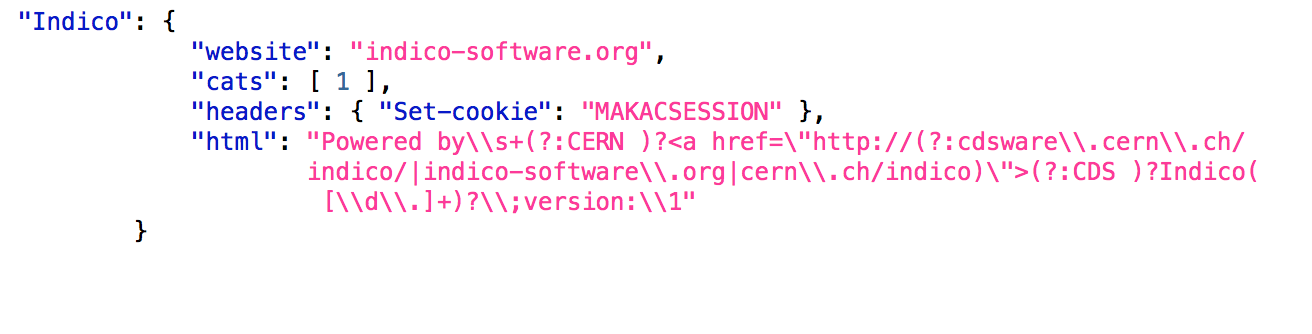
\includegraphics[width=1.0\textwidth]{indico}
  \caption{Indico Detection Rule}
  \label{figure:indico}
\end{figure}
 
\subsection{Detection Scripts}
Over the years, the CERN Computer Security Team has developed individual scripts. Most of these scripts are short security tests to check for an emerging vulnerability (e.g. Heartbleed) on CERN resources. Additionally, some scripts detect misconfigurations (e.g. empty landing pages) on web servers that could threaten the security of CERN resources. Currently, CERN can detect the following vulnerabilities, using detection scripts:
\begin{itemize}
\item \textbf{Heartbleed} - The device is vulnerable to OpenSSL Heartbleed vulnerability
\item \textbf{SSL2 Check}: - SSL version 2 is enabled
\item \textbf{SSL3 Check}: - SSL version 3 is enabled
\item \textbf{Weak Cipher} - The server is using an insecure cipher
\item \textbf{Homepage Check} - The landing page is empty or the default landing page
\item \textbf{CouchDB Check} - The CouchDB\footnote{Apache open source NoSQL database that can be accessed from web} database is protected
\item \textbf{Expired Certificate} - The server is using an expired certificate
\item \textbf{Self-signed Certificate} - The server is using a self-signed certificate
\item \textbf{Non-valid Certificate} - The server is using a certificate that is not valid for the domain
\item \textbf{Non-trusted Certificate} - The server is using a certificate that is not trusted
\item \textbf{Wildcard Certificate} - The server is using a wildcard certificate
\item \textbf{Basic HTTP Authentication} - The website or web server is using Basic HTTP Authentication
\item \textbf{OpenSSL CCS Injection} - The device is vulnerable to the OpenSSL Change Cipher Spec (CCS) injection vulnerability

\end{itemize}



\section{Objectives}
\paragraph{}
The main objective of this project is to automate --as much as possible-- the procedures for detecting vulnerable web applications. We would like to take advantage of publicly available vulnerability sources to detect CERN resources that use vulnerable third party products. Another objective of the project is to facilitate scanning CERN resources for critical vulnerabilities in emergency cases, specially when a vulnerability is not specific to a certain, detectable product. This project focuses on detection of vulnerable web applications remotely, more specifically when a new vulnerability emerges.


























\chapter{Vulnerability Notification Tool}
\label{vulnerability-notification-tool}
\thispagestyle{empty}

\section{Motivation}
Every day new vulnerabilities and security updates are announced. Some of these vulnerabilities affect CERN websites or web servers and could be critical. Therefore, it is important to learn about them as soon as possible and notify the owners of the affected resources to take necessary actions, i.e. patch or update their resource. The current procedure in the CERN Computer Security Team for managing vulnerabilities is as follows:
\begin{enumerate}
\item Getting informed about vulnerabilities from various sources by monitoring public databases, project mailing lists, security mailing lists, Twitter accounts, blogs, etc.
\item Deciding if a vulnerability is worth investigating and is likely to affect CERN (human decision).
\item In case of vulnerabilities related to web applications, reviewing the output of WAD on all CERN websites and web servers, in order to get a list of resources that could be affected.
\item Sending notifications to the resource owners after making sure that the resource is in fact vulnerable, i.e. runs a vulnerable version or has a vulnerable configuration.
\end{enumerate}

The main goal of the Vulnerability Notification Tool (VNT) we developed is to automate this procedure as much as possible and optimize each step of the process. Staying up-to-date with vulnerability sources and announcements is a time consuming task and it is hard to know if one is monitoring the best sources. With the current procedure, it is easy to overlook some vulnerabilities that are important for CERN, but do not create much noise in the public. 
On the other hand, so many vulnerabilities are published every day that it is impossible to investigate every single one of them even if we know about all of them.

Figure \ref{figure:vulns_per_year}\footnote{Picture taken from \url{http://web.nvd.nist.gov/view/vuln/statistics-results?adv_search=true&cves=on&pub_date_start_month=0&pub_date_start_year=2000&pub_date_end_month=11&pub_date_end_year=2014}} shows the trend in the number of vulnerabilities published in the last 15 years. Apparently, 2014 with almost 8000 vulnerabilities has been the worst year so far for security. Due to the ever increasing volume of public vulnerability reports, the CVE MITRE vulnerability repository has even updated the CVE-ID syntax since January 2015. The new syntax, unlike the previous 4-digit one, allows identifying an unlimited number of vulnerabilities each year.\footnote{\url {https://cve.mitre.org/cve/identifiers/syntaxchange.html}} 
\paragraph{}
VNT tries to save the CERN Computer Security Team's time by filtering out the non-critical vulnerabilities or the vulnerabilities that do not affect CERN, so that more time can be spent on remediation of the remaining ones.


\begin{figure}[h!]
\label{figure:vulns_per_year}
  \centering
    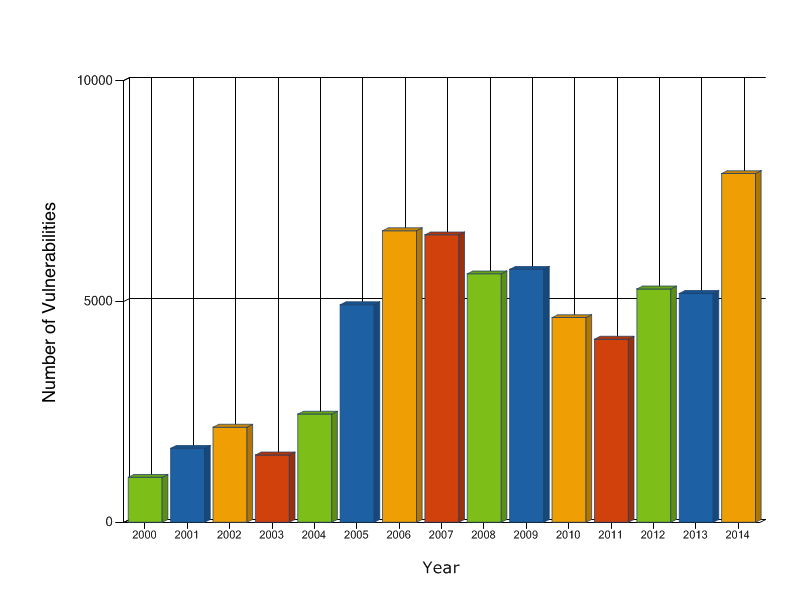
\includegraphics[width=1.0\textwidth]{vulns_per_year}
  \caption{Number of Vulnerabilities Discovered in Each Year (From NVD)}
  
\end{figure}

%\section{Related Work}
%
%\subsection{Cassandra}

\section{Source Evaluation}
\label{source_evaluation}
There are plenty of public sources that announce vulnerabilities or maintain a database of all vulnerabilities over the years. The performance of VNT very much depends on the quality of the source it is using. Obviously, it is not possible to find a perfect source. For example, there is a trade-off between the speed of publishing the vulnerabilities and the accuracy of the information published; hence, it is crucial to know the needs of the organization and choose the most suitable source.

\subsection{Approach}
In order to evaluate vulnerability sources, the following factors have been considered:
\begin{enumerate}
\item \textbf{Completeness}: Does the source contain all the vulnerabilities that CERN would probably care about? 
\item \textbf{Speed}: How long, since the disclosure, does it take for a vulnerability to be published?
\item \textbf{Information Quality}: What information (e.g. severity level, exploits, solutions, etc.) about a vulnerability is published?
\item \textbf{Parsable Feed}: Does the source provide a parsable feed that can be downloaded and updated automatically?
\item \textbf{Cost}: Is the source free for public use? If not, how much does it cost?
\end{enumerate} 

Table \ref{table:sample_vulns} contains 6 vulnerabilities published over the last few months. These vulnerabilities have been used as case studies to evaluate completeness and speed of different sources. These vulnerabilities were of great importance for CERN and can be a good indicator of how well a source fits CERN needs.
\begin{table}
\begin{center}
\resizebox{1\textwidth}{!}{

    \begin{tabular}{ | c | c | c| }
    
    \hline
    \hhline{|*3-}
	\rowcolor{LightBlue}    
    \textbf{Vulnerability} & \textbf{CVE-ID} & \textbf{Disclosure Date} 
    %& Summary 
    \\ \hline
    GitLab groups API & CVE-2014-8540 & 30.10.2015
%     & The vulnerability allows a guest user to delete the owner of a group and to assign any other member as owner through the groups API.
      \\ \hline
    Wordpress 4.0.1 Security Release & CVE-2014-9032(*)  & 20.11.2014
    % & XSS vulnerability allows remote attackers to inject arbitrary web script or HTML via unspecified vectors.[...]\footnote{\url{https://wordpress.org/news/2014/11/wordpress-4-0-1/}} 
    \\ \hline
    Drupal SQL injection
 & CVE-2014-3704
 & 15.10.2014 
 %& The vulnerability allows remote attackers to conduct SQL injection attacks via an array containing crafted keys
  \\
    \hline

 Poodle
 & CVE-2014-3566
 & 14.10.2014
 %& The SSL protocol 3.0 allows man-in-the-middle attackers to obtain clear text data via a padding-oracle attack
  \\
    \hline

Twiki Remote Code Execution
 & CVE-2014-7236
 & 09.10.2014
 %& The debugenableplugins request parameter allows arbitrary Perl code execution.  
 \\
    \hline

ShellShock
 & CVE-2014-6271
 & 24.09.2014
 %& Via certain applications, a local or remote attacker may inject shell commands, allowing local privilege escalation or remote command execution depending on the application vector. 
  \\
    \hline

    \end{tabular}
    }
    \caption{Sample vulnerabilities}
    \label{table:sample_vulns}
     \footnotesize{(*) Multiple vulnerabilities (CVE-2014-9032, CVE-2014-9033, CVE-2014-9034, CVE-2014-9035, CVE-2014-9036, CVE-2014-9037) were released at the same time.}
   \end{center}
   
\end{table}


\subsection{Vulnerability Sources}
\label{vuln_sources}
Plenty of mailing lists, databases, vulnerability sources, etc. are available online. Each of these sources provides different types of information for different purposes. A part of this project was to do some research on these different sources and compare them with respect to CERN needs. In this section, we will go through a summary of the sources that were evaluated. 
\begin{itemize}
\item \textbf{Natinal Vulnerability Database (NVD)}\footnote{\url{https://nvd.nist.gov/}}: The U.S. government repository of standards-based vulnerability management data.
\item \textbf{Open Sourced Vulnerability Database (OSVDB)}\footnote{\url{http://www.osvdb.org}}: An independent and open sourced\footnote{The data is collected from publicly available sources} web-based vulnerability database created for the security community. 
\item \textbf{CVE Details}\footnote{\url{http://www.cvedetails.com/}}: A web interface providing CVE vulnerability data and statistics about vendors and products.
\item \textbf{Secunia Vulnerability Intelligence Manager (VIM)}\footnote{\url{http://secunia.com/vulnerability_intelligence}}: An online service providing a filtered feed of verified vulnerability intelligence in real-time.

\end{itemize}
\paragraph{Completeness and Speed}
Table \ref{table:source_speed} illustrates the publication date of sample vulnerabilities on individual sources. If a source is missing a particular vulnerability the corresponding cell is empty. Using this table, we can compare the completeness and speed of different sources. Note that in each row, the fastest source is marked in green, the slowest in red and the average ones are marked in yellow. Taking a glance at the table, we can realize that OSVDB has the highest publication speed and is the most complete source.

\begin{table}
\begin{center}
\resizebox{1\textwidth}{!}{

    \begin{tabular}{ | c || c | c | c | c | c | c |}
    
    \hline
	
      Vulnerability(*) & \textbf{NVD}  &  \textbf{OSVDB} & \textbf{CVE Details} & \textbf{Secunia VIM} 
	\\ 
	\hline  
%	\hhline{|*5-}  
	\textbf{GitLab} & \multicolumn{1}{c|}{\cellcolor{red!25}} & \multicolumn{1}{c|}{\cellcolor{green!25} 31.10.2014} & \multicolumn{1}{c|}{\cellcolor{red!25}} & \multicolumn{1}{c|}{\cellcolor{red!25}} 
    \\ 
	\hline   
%	\hhline{~|*4-} 
	 \textbf{Wordpress} & \multicolumn{1}{c|}{\cellcolor{yellow!25} 25.10.2014} & \multicolumn{1}{c|}{\cellcolor{green!25} 21.10.2014} & \multicolumn{1}{c|}{\cellcolor{red!25}} & \multicolumn{1}{c|}{\cellcolor{green!25} 21.10.2014} 
	  \\ 
	\hline
%	\hhline{~|*4-} 
	 \textbf{Drupal} & \multicolumn{1}{c|}{\cellcolor{yellow!25}17.10.2014} & \multicolumn{1}{c|}{\cellcolor{yellow!25}17.10.2014} & \multicolumn{1}{c|}{\cellcolor{yellow!25}17.10.2014} & \multicolumn{1}{c|}{\cellcolor{green!25}16.10.2014}
	  \\ 
	\hline
%	\hhline{~|*4-} 
	 \textbf{Poodle} & \multicolumn{1}{c|}{\cellcolor{yellow!25}16.10.2014} & \multicolumn{1}{c|}{\cellcolor{yellow!25}19.10.2014} & \multicolumn{1}{c|}{\cellcolor{yellow!25}16.10.2014} & \multicolumn{1}{c|}{\cellcolor{green!25}15.10.2014}
	  \\ 
	\hline 
%	\hhline{~|*4-} 
	 \textbf{Twiki} & \multicolumn{1}{c|}{\cellcolor{red!25}} & \multicolumn{1}{c|}{\cellcolor{green!25} 09.10.2014} & \multicolumn{1}{c|}{\cellcolor{yellow!25} 11.10.2014} &\multicolumn{1}{c|}{\cellcolor{red!25}}
	  \\ 
	\hline 
%	\hhline{~|*4-} 
	 \textbf{ShellShock} & \multicolumn{1}{c|}{\cellcolor{green!25}25.09.2014} & \multicolumn{1}{c|}{\cellcolor{green!25}25.09.2014} & \multicolumn{1}{c|}{\cellcolor{green!25}25.09.2014} &\multicolumn{1}{c|}{\cellcolor{green!25} 25.09.2014} 
	 \\
	 \hline
    %\hhline{|*5-}
     
%\hhline{~~|-|~|-|}
%Critical\textsuperscript{*} & 190  & \multicolumn{1}{|c||}{\cellcolor{green!25}9}  & 622  & \multicolumn{1}{|c|}    
\end{tabular}
}
    \caption{Vulnerability Publication Dates}
    \label{table:source_speed}
    \footnotesize{(*) For the complete name of the vulnerability refer to Table \ref{table:sample_vulns}}
   \end{center}
    \end{table}


\paragraph{Information Quality}
The comparison of the information quality in different sources is illustrated in Table \ref{table:info_quality}. All sources have almost the same quality of the information. It is true that NVD provides less information than the other sources, but it is still providing most of the important fields that we are interested in. 



\begin{table}
\begin{center}
\resizebox{1\textwidth}{!}{

    \begin{tabular}{ | c || c | c | c | c | c | c |}
    
    \hline
	 
      Data & \textbf{NVD}  &  \textbf{OSVDB} & \textbf{CVE Details} & \textbf{Secunia VIM} 
	\\ 
	\hline  
%	\hhline{~|*4-}  
	\textbf{Description} & \multicolumn{1}{c|}{\cellcolor{green!25}\cmark} & \multicolumn{1}{c|}{\cellcolor{green!25}\cmark}
	& \multicolumn{1}{c|}{\cellcolor{green!25}\cmark}& \multicolumn{1}{c|}{\cellcolor{green!25}\cmark}
    \\ 
	\hline   
%	\hhline{~|*4-} 
	 \textbf{Severity} & \multicolumn{1}{c|}{\cellcolor{green!25}\cmark} & \multicolumn{1}{c|}{\cellcolor{green!25}\cmark}
	& \multicolumn{1}{c|}{\cellcolor{green!25}\cmark}& \multicolumn{1}{c|}{\cellcolor{green!25}\cmark}
	  \\ 
	\hline
%	\hhline{~|*4-} 
	 \textbf{Product} & \multicolumn{1}{c|}{\cellcolor{green!25}\cmark} & \multicolumn{1}{c|}{\cellcolor{green!25}\cmark}
	& \multicolumn{1}{c|}{\cellcolor{green!25}\cmark}& \multicolumn{1}{c|}{\cellcolor{green!25}\cmark}
	  \\ 
	\hline
%	\hhline{~|*4-} 
	 \textbf{Exploits} & \multicolumn{1}{c|}{\cellcolor{red!25}\xmark} & \multicolumn{1}{c|}{\cellcolor{red!25}\xmark}
	& \multicolumn{1}{c|}{\cellcolor{green!25}\cmark}& \multicolumn{1}{c|}{\cellcolor{red!25}\xmark}
	  \\ 
	\hline 
%	\hhline{~|*4-} 
	 \textbf{Solution} & \multicolumn{1}{c|}{\cellcolor{red!25}\xmark} & \multicolumn{1}{c|}{\cellcolor{green!25}\cmark}
	& \multicolumn{1}{c|}{\cellcolor{red!25}\xmark}& \multicolumn{1}{c|}{\cellcolor{green!25}\cmark}
	  \\ 
	\hline 
%	\hhline{~|*4-} 
	 \textbf{Vulnerability Type} & \multicolumn{1}{c|}{\cellcolor{green!25}\cmark} & \multicolumn{1}{c|}{\cellcolor{green!25}\cmark}
	& \multicolumn{1}{c|}{\cellcolor{green!25}\cmark}& \multicolumn{1}{c|}{\cellcolor{green!25}\cmark}
	 \\
	 \hline	 

    %\hhline{|*5-}
     
%\hhline{~~|-|~|-|}
%Critical\textsuperscript{*} & 190  & \multicolumn{1}{|c||}{\cellcolor{green!25}9}  & 622  & \multicolumn{1}{|c|}    
\end{tabular}
}
    \caption{Source Information Quality}
    \label{table:info_quality}
   \end{center}
    \end{table}
    
    
    
    
    
\paragraph{Parsable Feed and Cost}
NVD provides free XML data feeds. OSVDB provides information via the web interface as a free resource for the community. Alternate methods of obtaining the data such as API or exports are no longer supported via OSVDB and are offered by Risk Based Security as a commercial product, called VulnDB API. CVE Details offers JSON feeds for the vulnerabilities, but unfortunately, the feeds are not complete and they do not contain vulnerable product information which is one of the most important fields for the purpose of VNT. Secunia VIM is also a commercial product\footnote{A trial account was used for evaluation.} and it provides vulnerability information via a web portal. It is possible to download XML description of vulnerabilities limited to the last 72 hours; however, the main focus of VIM is on vulnerability management through the graphical web interface. 
    
   

\subsection{Conclusion}
Table \ref{table:source_evaluation} illustrates a summary of the source evaluation results. Like the two previous tables, green cells show a high evaluated score, yellow represents an average score and red is marking an unacceptable score. Downloading the latest vulnerability information automatically is one of the requirements of VNT. In addition, VNT is supposed to analyze the vulnerability data to filter out the non-critical vulnerabilities and those unrelated to CERN. Therefore, it is important to have the vulnerability information in a structured and parsable format. 
The only sources that provide a useful parsable feed are NVD, OSVDB (the feed offered commercially under the name VulnDB API) and Secunia VIM. 
\paragraph{}
Secunia VIM focuses on vulnerability management, assuming that there is a human using its portal and taking necessary actions. An XML description of vulnerabilities from the last 72 hours can be downloaded as an additional functionality, but unlike VulnDB there is no API access to the feed. 
\paragraph{}
NVD was the source we finally used as the input to VNT. The two other solutions are commercial, and their additional benefits did not, in our case, justify their respective costs. 
\paragraph{}
Although it has not been a decision factor, it is worth mentioning that vulnerability databases use different methods of abstraction. Some, like NVD, keep one entry per vulnerability, while some others, like Secunia VIM, create multiple entries for the same vulnerability, because there are different patches available (for different operating systems, for example).

   
    \begin{table}
\begin{center}
\resizebox{1\textwidth}{!}{
    \begin{tabular}{ | c || c | c | c | c | c | c |}
    
    \hline
	 
      Data & \textbf{NVD}  &  \textbf{OSVDB} & \textbf{CVE Details} & \textbf{Secunia VIM} 
	\\ 
	\hline  
%	\hhline{~|*4-}  
	\textbf{Completeness} & \multicolumn{1}{c|}{\cellcolor{yellow!25}\cmark} & \multicolumn{1}{c|}{\cellcolor{green!25}\cmark}
	& \multicolumn{1}{c|}{\cellcolor{yellow!25}\cmark}& \multicolumn{1}{c|}{\cellcolor{yellow!25}\cmark}
    \\ 
	\hline   
%	\hhline{~|*4-} 
	 \textbf{Speed} & \multicolumn{1}{c|}{\cellcolor{green!25}\cmark} & \multicolumn{1}{c|}{\cellcolor{green!25}\cmark}
	& \multicolumn{1}{c|}{\cellcolor{green!25}\cmark}& \multicolumn{1}{c|}{\cellcolor{green!25}\cmark}
	  \\ 
	\hline
%	\hhline{~|*4-} 
	 \textbf{Information Quality} & \multicolumn{1}{c|}{\cellcolor{green!25}\cmark} & \multicolumn{1}{c|}{\cellcolor{green!25}\cmark}
	& \multicolumn{1}{c|}{\cellcolor{green!25}\cmark}& \multicolumn{1}{c|}{\cellcolor{green!25}\cmark}
	  \\ 
	\hline
	 \textbf{Feed Completeness} & \multicolumn{1}{c|}{\cellcolor{green!25}\cmark} & \multicolumn{1}{c|}{\cellcolor{green!25}\cmark(*)}
	& \multicolumn{1}{c|}{\cellcolor{red!25}\xmark}& \multicolumn{1}{c|}{\cellcolor{green!25}\cmark}
	 \\
	 \hline
	 
	 \textbf{Feed Cost} & \multicolumn{1}{c|}{\cellcolor{green!25}Free} & \multicolumn{1}{c|}{\cellcolor{yellow!25}Commercial(*)}
	& \multicolumn{1}{c|}{\cellcolor{green!25}Free}& \multicolumn{1}{c|}{\cellcolor{yellow!25}Commercial}
	 \\
	 \hline
    %\hhline{|*5-}
     
%\hhline{~~|-|~|-|}
%Critical\textsuperscript{*} & 190  & \multicolumn{1}{|c||}{\cellcolor{green!25}9}  & 622  & \multicolumn{1}{|c|}    
\end{tabular}
}
    \caption{Source Evaluation}
    \label{table:source_evaluation}
    \footnotesize{(*) Under the name VulnDB}
   \end{center}
    \end{table}


\section{National Vulnerability Database}
NVD is the U.S. government repository of standards-based vulnerability management data and contains 68054 CVE vulnerabilities. It is recommended by the MITRE Corp. hosting CVE\footnote{https://cve.mitre.org/} to obtain information about a vulnerability severity rating, fix information, vulnerable software versions, etc. 
 
\subsection{Data Feeds}
The entire NVD can be downloaded from its web page for free and for public use. The XML vulnerability feed contains security related software flaws. Each vulnerability in the file includes a description and associated reference links from the CVE dictionary feed, as well as a CVSS base score\footnote{Common Vulnerability Scoring System is a standard measurement system for rating the severity of IT vulnerabilities}, vulnerable product configuration, and weakness categorization. The feed provides vulnerability information since 1999 (one file for each year, except that the file from 2002 includes all vulnerabilities published in 2002 and before). In addition, there is a ``recent'' feed, listing recently published vulnerabilities and a ``modified" feed, which includes the ``recent" feed plus all recently modified vulnerabilities, where ``recently" means the previous eight days. The feeds are updated approximately every two hours.


\subsection{Challenges}
\subsubsection{Downloading}
The ``modified" feed from NVD contains the latest vulnerabilities published or modified in the last eight days. Obviously, if the tool is not used for more than eight days, it will definitely miss some updates. This issue can be fixed by looking at the yearly feeds and detecting if a vulnerability information has changed in those feeds since the last execution. Anyhow, it was decided that the NVD feed will be consulted at least once a day and therefore, there is no need for consulting the yearly feeds. 
\paragraph{}
Another point worth mentioning is that NVD keeps no record of the changes that happen in vulnerability data. It is impossible to see how a vulnerability has changed over time, because new data are always overwriting the old ones. VNT does not care about any intermediate changes in a vulnerability information between two subsequent executions, but for a complete evaluation of the tool and in order to be able to simulate the tool over a period of time, we kept a local copy of the ``modified" feed, downloaded daily since October 31\textsuperscript{th}, 2014. 
\subsubsection{Modification Date}
Since NVD provides the last modified date as one of the fields in the vulnerability information, the easiest way to find the vulnerabilities that have changed since the last execution of the tool, would be to compare their last modified time with the time of the last execution. However, this method will not work because the last modified time reported by NVD is not always correct. Imagine a vulnerability X published at time t$_{\text{0}}$. If we look at the NVD feed at time t$_{\text{2}}$ we see that the last modified time for the vulnerability is t$_{\text{0}}$, which means that the vulnerability has not changed since its publication. Now we may look at the vulnerability at time t$_{\text{3}}$ and to our surprise, we may see that the last modified time is t$_{\text{1}}$  (t$_{\text{0}}$<t$_{\text{1}}$<t$_{\text{2}}$). This means that although the vulnerability information was updated at time t$_{\text{1}}$, the update was not visible for sometime and we missed it at time t$_{\text{2}}$. If we compare the last modified time (t$_{\text{1}}$) to the last execution time (t$_{\text{2}}$) we might decide to ignore the vulnerability and assume it has not changed. 
\paragraph{}
A script was written to check for existence of similar cases in NVD feeds and many instances of this controversy were found. For example, on 05.11.2014 the last modified time of CVE-2012-5500 was reported as 03.11.2014 and if we check for the same vulnerability on 06.11.2014 we get the last modified time as 04.11.2014. In addition, one can observe that sometimes the details of a vulnerability, such as its CVSS score change without changing the last modified field. Due to these problems, it was decided to ignore the last modified time field completely and use the following alternative solution to find updated vulnerabilities:
\paragraph{}
The tool stores a local copy of vulnerability information (one JSON file per vulnerability). For each vulnerability in the downloaded feed we look at our local version of that vulnerability. If there is no local version, the vulnerability is reported as newly published and its data is stored locally, otherwise we compare the local version with the new data, report the changes and update the stored data.
\paragraph{}
This solution solves the modification date problem and makes it possible to report what exactly has changed in a vulnerability. 

\subsubsection{Vulnerable Configuration}
In addition to the list of vulnerable software packages, NVD provides a list of vulnerable configurations. For example, if Safari 5.0.5 is vulnerable only on Mac OS X 10.5.8 the vulnerable-software-list would contain Safari 5.0.5 but no information about the operating system. In this case, it would be useful to extract the configuration data from NVD and use it to make sure when a resource is vulnerable. Given the scope of this project, unavailability of configuration specifications on CERN resources and the fact that only a few vulnerabilities are bound to a specific configuration, we decided to ignore this field and only consider the products from the vulnerable-software-list field. 




\section{Product Name Matching}
\label{name_matching}
The next step after extracting new and modified vulnerabilities is to find the CERN resources that might be affected by these vulnerabilities. As an intermediate step, it is important to find which WAD names\footnote{Names that WAD uses to report detected technologies, such as Apache, Microsoft SharePoint, PHP-Fusion, etc.} are affected by each vulnerability. If we know about the affected WAD names, finding the affected resources is an easy task that just requires going through WAD output on all websites and web servers at CERN and reporting the URLs of all those including the affected WAD names. 

\subsubsection{Common Platform Enumerations}
NVD is using the Common Platform Enumeration syntax to list the vulnerable softwares for each vulnerability. The Common Platform Enumeration (CPE) is a structured naming schema for IT systems, platforms and packages. It aims at providing a formal, consistent and uniform naming schema, so that the community members are able to generate names for new IT platforms in a consistent and predictable way.\footnote{\url{https://nvd.nist.gov/cpe.cfm}} This will facilitate automation in security practices. CPE is based on the generic syntax for Uniform Resource Identifiers. A standard CPE name is in the format of \texttt{cpe:/\{type\}:\{vendor\}:\{name\}:\{version\}}. The type of a platform can be either hardware (h), operating system (o), or application environment (a). Some CPEs can contain more components to provide additional information. Table \ref{table:sample_cpes} contains some examples of CPE names. 
%todo reference to cpe spec
\begin{table}
\begin{center}
\resizebox{1\textwidth}{!}{

    \begin{tabular}{ | c | c | }
    
    \hline
	 \hhline{|*2-}
	%\rowcolor{LightBlue}   
     \multicolumn{1}{|c|}{\cellcolor{LightBlue}\textbf{CPE}} &  \multicolumn{1}{|c|}{\cellcolor{LightBlue}\textbf{Description}}  
    \\ \hline
    % cpe:/o:microsoft:windows_xp:::home
    % cpe:/h:samsung:galaxy_note_2:-"
    % cpe:/a:wordpress:wordpress:1.0
    \multirow{3}{*}{\texttt{cpe:/h:samsung:galaxy\_note\_2:-}} & Samsung Galaxy Note 2 \\ & (Hardware) \\ & 
        \\ \hline
   \multirow{3}{*}{\texttt{cpe:/o:microsoft:windows\_xp:home}} & Microsoft Windows XP \\ & Home Edition \\ & Operating System
        \\ \hline
         \multirow{3}{*}{\texttt{cpe:/a:wordpress:wordpress:1.0}} &  \\ & Wordpress 1.0 \\ & 
        \\ \hline
    \end{tabular}
    }
    \caption{CPE Examples}
    \label{table:sample_cpes}
   \end{center}
    
\end{table}

In this project we only care about vulnerabilities that affect operating systems or applications, therefore, we can ignore the hardware related vulnerabilities when mapping CPE to WAD names. As you can see in the examples, the first three components of the CPE (after the type indicator) are the ones that describe the vulnerable software in the format of \texttt{\{vendor\}:\{name\}:\{version\}}.
 

\subsubsection{WAD Product Names}
%TODO: refer to section wad
As already described in section \ref{sec:tools}, WAD uses detection rules coming from Wappalyzer which is an open source browser plugin with a community of over 100 contributors. Wappalyzer relies on its contributors' common sense to choose a meaningful name for each technology it detects and therefore there is no standard syntax for Wappalyzer names. As of the time of writing this thesis, Wappalyzer detects 707 technologies from 50 different categories.


\subsection{Approach}

There are two approaches that we can follow to do the mapping from CPE names to WAD names:
\begin{enumerate}
\item \textbf{Static Mapping}: In static mapping we would need to create a dictionary that lists all WAD names for each CPE name. Generating this dictionary for the first time would be a time consuming manual work, but would guarantee a high level of accuracy. This dictionary needs to be updated whenever there is a new WAD name or CPE name. 
\item \textbf{Dynamic Mapping}: In the dynamic mapping approach we would need to design an algorithm that would find WAD names for a CPE name on the fly. By using this approach, there would be no need for any maintenance, except optionally improving the matching algorithm over time. But the price we pay with dynamic mapping is lower accuracy, i.e more false positives (wrongly matching a CPE name to a WAD name) and false negatives (missing a match between a CPE name and a misleading but actually corresponding WAD name).  
\end{enumerate} 



\subsubsection{Challenges}
The lack of a standard naming approach in Wappalyzer and consequently in WAD, makes it difficult to match CPE names to WAD names. On the other hand, CPE itself is not 100\% consistent and sometimes for the same application, one can find multiple CPE names,e.g. \texttt{cpe:/a:django\_piston\_project:django\_piston:0.2.2.0}, \texttt{cpe:/a:djangoproject:django\_piston:0.2.2.0} and \texttt{cpe:/a:djangoproject:piston:0.2.2.0} are available CPE names that refer to the same application.
\paragraph{}
There is an official CPE dictionary available online that is supposed to provide an agreed upon list of official CPE names\footnote{\url{https://nvd.nist.gov/cpe.cfm}}. Unfortunately, one can notice that many of the CPE names that appear on NVD vulnerability feeds are not present in this dictionary and therefore there is no way of knowing which CPEs we are going to find in vulnerability feeds, in advance. Considering the CPE dictionary as well as all the vulnerabilities published on NVD, currently there are 33,615 unique CPE names (vendor and product names, ignoring other components such as version). Table \ref{table:cpe_wad_mapping} tries to show how challenging it might be to find equivalent WAD names of a CPE name.

\begin{table}
\begin{center}
\resizebox{1\textwidth}{!}{

    \begin{tabular}{ | c | c | }
    
    \hline
	 \hhline{|*2-}
%	\rowcolor{LightBlue}   
    \multicolumn{1}{|c|}{\cellcolor{LightBlue}\textbf{CPE}} & \multicolumn{1}{|c|}{\cellcolor{LightBlue}\textbf{WAD Name}  }
    \\ \hline
    % cpe:/o:microsoft:windows_xp:::home
    % cpe:/h:samsung:galaxy_note_2:-"
    % cpe:/a:wordpress:wordpress:1.0
    \texttt{cpe:/a:adobe:coldfusion:8.0} & Adobe ColdFusion 
        \\ \hline
    \texttt{cpe:/a:yandex.metrics\_project:yandex\_metrics:1.0} & Yandex.Metrika
        \\ \hline
    \texttt{cpe:/a:woothemes:woocommerce\_plugin:2.1.0} & WooCommerce
        \\ \hline
 	\texttt{cpe:/a:djangoproject:django:1.6} & Django CMS 
        \\ \hline
    \texttt{cpe:/a:cagintranetworks:getsimple\_cms:1.0} & GetSimple CMS

        \\ \hline
    \texttt{cpe:/a:drupal:drupal:4.6.2} & Drupal
        \\ \hline
    \end{tabular}
    }
    \caption{CPE to WAD Name Mapping}
    \label{table:cpe_wad_mapping}
   \end{center}
    
\end{table}



\subsection{Algorithm}


Considering the challenges we discussed in the previous section and the likelihood of new CPE names appearing, as well as the overload of maintaining a dictionary of the mappings, it was decided to go for a dynamic mapping approach. 
\paragraph{}
Coming up with a matching algorithm that is complete and accurate at the same time is not an easy task. The more complete the matching is (higher recall), the less accurate it is going to be (lower precision). After analyzing the list of CPE names and WAD names and trying different matching algorithms, two algorithms were designed. Algorithm \ref{matching_algo} is an algorithm that matches a CPE name to a WAD name with a high level of accuracy. A match is found only if the WAD name is the combination of CPE product and vendor names or it equals the CPE product name. Algorithm \ref{matching_algo_2} adds more matches, but has a lower level of accuracy. The user can choose to use only algorithm \ref{matching_algo} for a higher precision or both algorithms together to get a higher recall rate. Note that both algorithms receive the CPE and WAD names in lower case with leading and trailing white spaces removed. In the first algorithm these names are being normalized before they are used, which means that all punctuation marks and white spaces inside the names are removed.  
%\begin{framed}
\begin{algorithm}
\begin{algorithmic}
\STATE $matches\gets$ array()
\STATE $cpe\_name\gets$ normalize($cpe\_vendor$)+normalize($cpe\_product$)

\FORALL{$wad\_name \in wad\_names$}

\IF{normalize($wad\_name$)$ = cpe\_name$}
		\STATE $matches+=wad\_name$
		\ELSIF{normalize($wad\_name$)=normalize($cpe\_product$)}
		\STATE $matches+=wad\_name$
		
		\ENDIF
\ENDFOR
\RETURN $matches$
%
%
%
%\STATE $wad\_normalized\_names\gets$ normalize($wad\_names$)
%\STATE $N\gets$ NumberOfTweets($D$)
% \FORALL{$wad\_name \in wad\_names$}
%  \STATE $N_c \gets$ Number of tweets in Class $c$
%  \STATE \begin{equation}prior(c) = \frac{N_c}{N}\end{equation}
%  \STATE $Tweets_c \gets $All Tweets in class $c$
%  \FORALL{$t \in V$}
%    \STATE $T_ct$ = No. of times term $t$ appeared in $Tweets_c$
%  \ENDFOR
%  \FORALL{$t \in V$}
%   \STATE \begin{equation}prob[t][c] = \frac{T_ct}{\sum^{t'}T_ct'+ 1}\end{equation}
%  \ENDFOR
%\ENDFOR

\end{algorithmic}
\caption{Name Matching Algorithm}
\label{matching_algo}
\end{algorithm}

\begin{algorithm}
\begin{algorithmic}
\STATE $matches\gets$ array()

\FORALL{$wad\_name \in wad\_names$}

\IF{normalize($wad\_name$)$ = $normalize($cpe\_vendor$)}
		\STATE $matches+=wad\_name$
		\ELSE
		\STATE $cpe\_name\gets cpe\_vendor + cpe\_product$ 
		\STATE $found\gets$ True
		\FORALL {$wad\_word \in wad\_name$}
		\IF { $wad\_word$ is not a word in $cpe\_name$}
		\STATE $found\gets$ False
		\ENDIF
		\ENDFOR
		\IF {$found=True$}
		\STATE $matches+=wad\_name$
		\ENDIF
		\ENDIF
\ENDFOR
\end{algorithmic}
\caption{Name Matching Algorithm}
\label{matching_algo_2}
\end{algorithm}


%\end{framed}
%\begin{algorithm}
%\caption{My algorithm}\label{euclid}
%\begin{algorithmic}[1]
%\Procedure{MyProcedure}{}
%\State $\textit{stringlen} \gets \text{length of }\textit{string}$
%\State $i \gets \textit{patlen}$
%\BState \emph{top}:
%\If {$i > \textit{stringlen}$} \Return false
%\EndIf
%\State $j \gets \textit{patlen}$
%\BState \emph{loop}:
%\If {$\textit{string}(i) = \textit{path}(j)$}
%\State $j \gets j-1$.
%\State $i \gets i-1$.
%\State \textbf{goto} \emph{loop}.
%\State \textbf{close};
%\EndIf
%\State $i \gets i+\max(\textit{delta}_1(\textit{string}(i)),\textit{delta}_2(j))$.
%\State \textbf{goto} \emph{top}.
%\EndProcedure
%\end{algorithmic}
%\end{algorithm}

%write an algorithm in latex 
 
\subsection{Evaluation}

\subsubsection{False Positives}
Very generic WAD names result into false positives. Table \ref{table:false_positives} shows some examples of the incorrect matches due to the generic WAD names. 
\begin{table}
\begin{center}
\resizebox{1\textwidth}{!}{

    \begin{tabular}{ | c | c | }
    
    \hline
	  \hhline{|*2-}
	%\rowcolor{LightBlue} 
    \multicolumn{1}{|c|}{\cellcolor{LightBlue}\textbf{CPE}} & \multicolumn{1}{|c|}{\cellcolor{LightBlue}\textbf{WAD Name}}  
    \\ \hline
    % cpe:/o:microsoft:windows_xp:::home
    % cpe:/h:samsung:galaxy_note_2:-"
    % cpe:/a:wordpress:wordpress:1.0
    \texttt{cpe:/a:20\_20\_applications:20\_20\_auto\_gallery} & Gallery
        \\ \hline
    \texttt{cpe:/a:altiris:dell\_client\_manager\_solution} & Dell
        \\ \hline
    \texttt{cpe:/a:redhat:cygwin} & Red Hat
        \\ \hline
    \end{tabular}
    }
    \caption{False Matches}
    \label{table:false_positives}
   \end{center}
%      \footnotesize{(*) \url{http://galleryproject.org/}\\
%      (**) Dell Printer Software \\
%      (***) Red Hat Operating System. It would be possible to prevent this false positive case by checking the catagory of the WAD name. The WAD category is \texttt{operating system}, while the CPE type is \texttt{application}, therefore, the matching should be refused. 
%      }
\end{table}

\subsubsection{False Negatives}
Finding false negatives, or in other words, missing matches, is more difficult than finding false positives because it involves going through both lists of WAD names and CPE names and finding matches manually to compare them with the algorithm output. Our algorithm might miss some mappings because of the  slight differences in product names, for example  \texttt{cpe:/a:yandex.metrics\_project:yandex\_metrics:1.0} will not be matched with \textit{Yandex.Metrika} or \texttt{cpe:/a:microsoft:outlook\_web\_access} will not match with \textit{Outlook Web App}. A possible improvement would be to use string distance algorithms to find similar names; however, that would make the algorithm much more complex.
\paragraph{}
Another cause of false negatives is inconsistency in word boundaries. Imagine a CPE name in the format of \texttt{cpe:/a:adobe:adobe\_coldfusion}; it will not match with \textit{Cold Fusion}, because Algorithm \ref{matching_algo_2} looks for the WAD name in CPE product name preserving the word boundaries. In this case, the algorithm could check for WAD names that are substrings of CPE names, but that approach would lead to many more false positives.


\section{Vulnerable Resources}
Now that we have a reasonably good idea of which WAD names are affected by a vulnerability, obtaining the list of vulnerable resources is quite an easy task, because the data is already available in WAD output. The Vulnerability Notification Tool only needs to load the output of WAD, group resources by the technologies they use and for each vulnerability report the resources that use the affected WAD name.
\\
\begin{figure}[H]
  \centering
    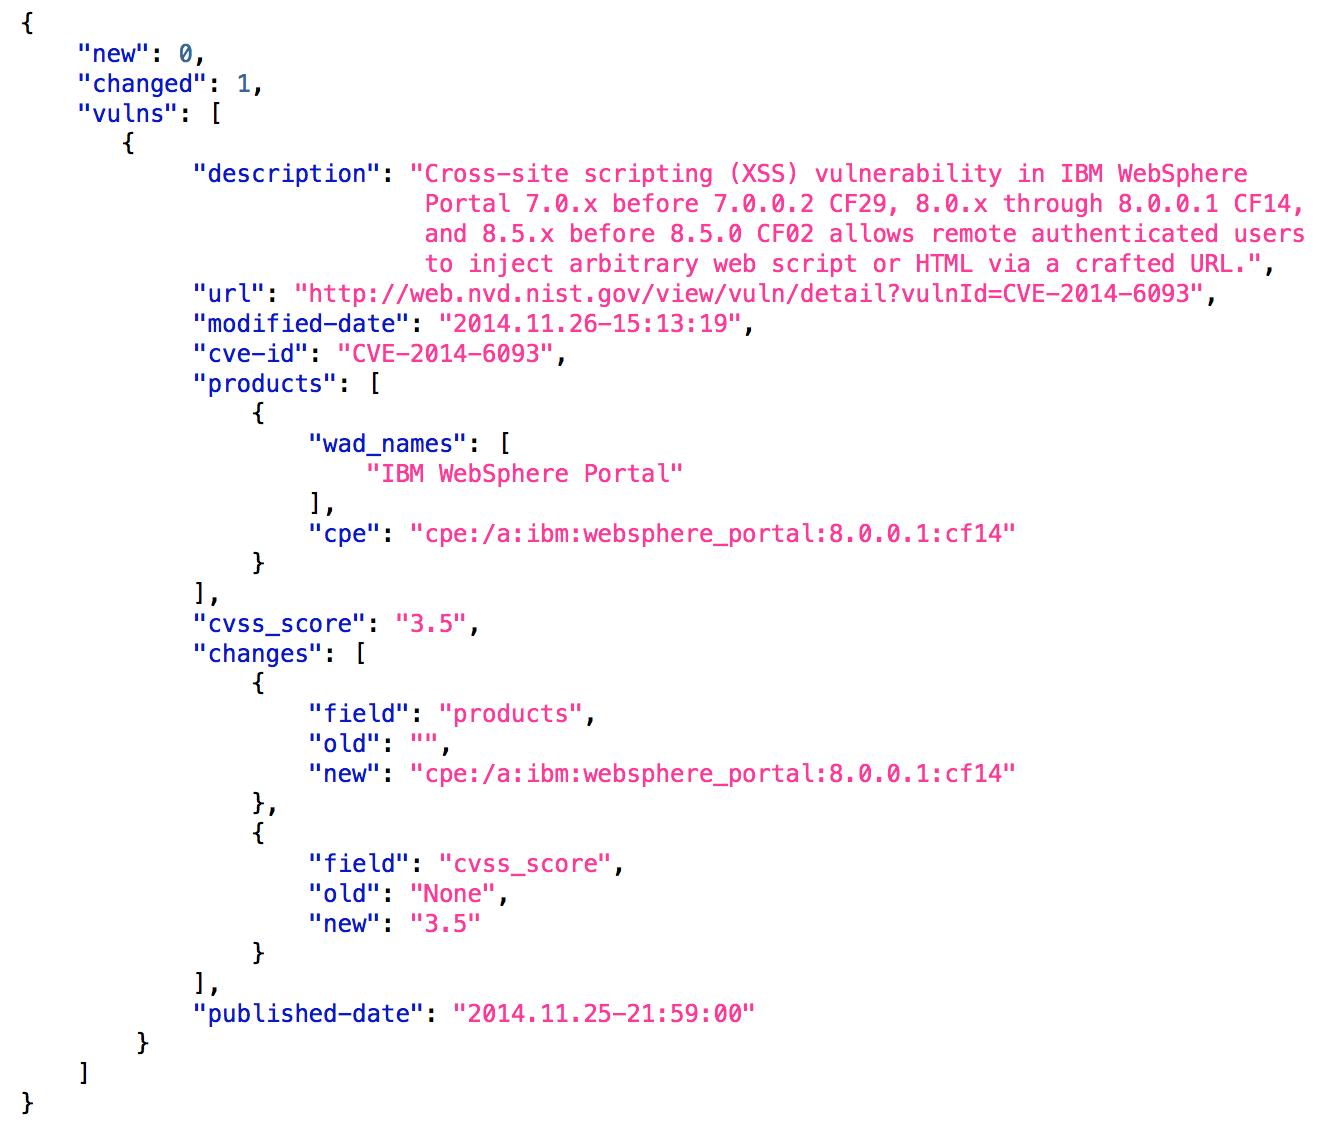
\includegraphics[width=1.0\textwidth]{json}
  \caption{Sample JSON output}
   \label{figure:json_output}
\end{figure}

\section{Output and Notifications}
VNT stores the results of its findings in JSON format. Figure \ref{figure:json_output} illustrates a sample of the stored JSON file. These files contain vulnerability information, updates and affected WAD names. They are easy to parse and can be used later for more analysis about vulnerabilities.
In addition, the tool sends email notifications to the CERN Computer Security Team members whenever there is a vulnerability that affects CERN and has a higher CVSS score than 6.0. Figure \ref{figure:email_output} shows one of the emails sent by the tool.
%todo: email photo

\begin{figure}[h!]
  \centering
    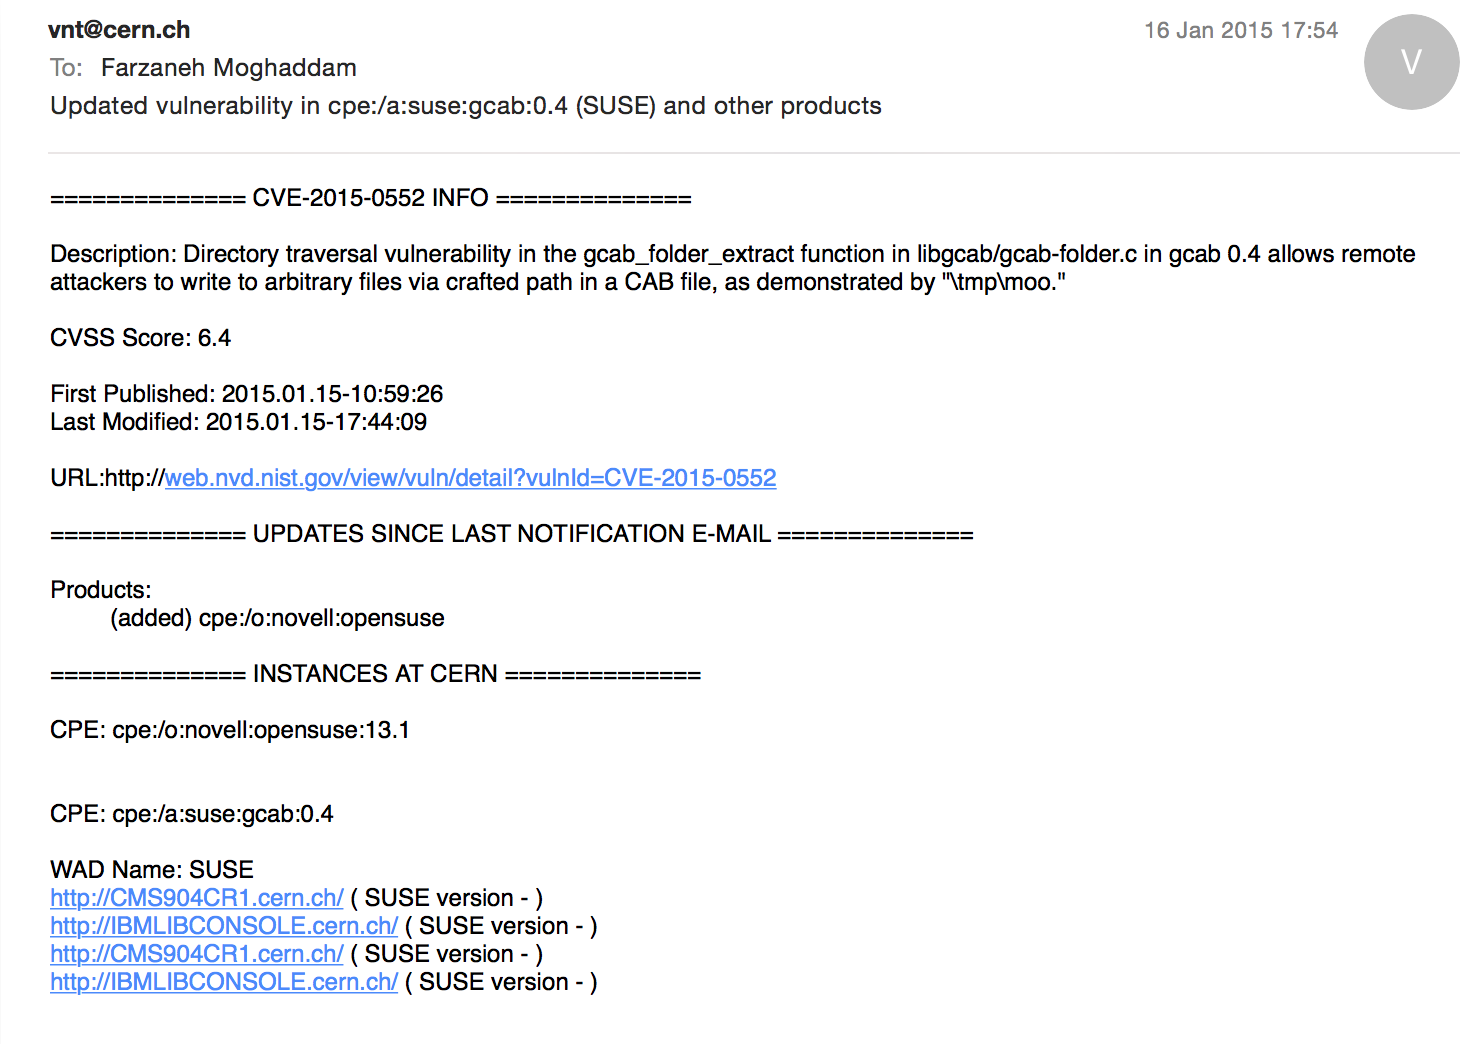
\includegraphics[width=1.0\textwidth]{email}
  \caption{Sample Notification Email}
 \label{figure:email_output}

\end{figure}


\section{Results}
The Vulnerability Notification Tool is a tool that downloads the latest ``modified" feed from NVD, finds the vulnerabilities that are newly published or have been changed since its last execution and for each of these vulnerabilities reports CVE-ID, description, CVSS score, published date and time, last modified date and time, and a list of affected software (vulnerable software in CPE format). In addition, the tool lists the URLs of the CERN websites and web servers that are likely to suffer from this vulnerability. Figure \ref{figure:vnt_arch} summarizes all functionalities of VNT and illustrates its architecture.

\begin{figure}[H]
  \centering
    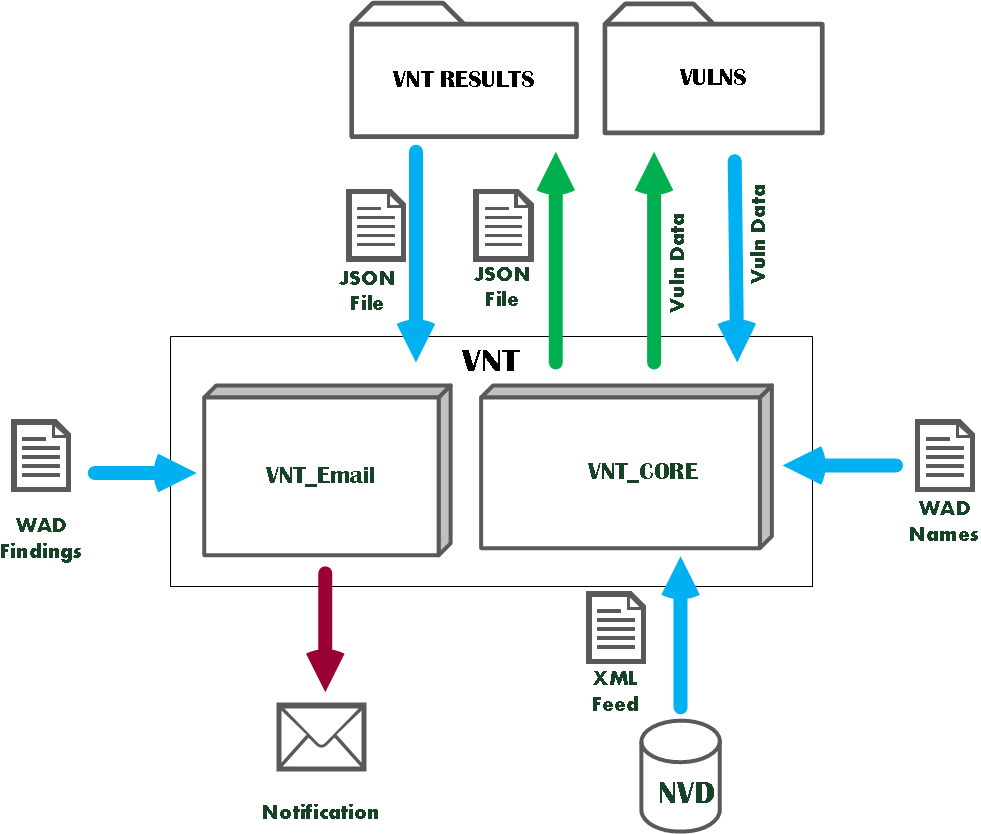
\includegraphics[width=1.0\textwidth]{vnt-architecture}
  \caption{VNT Architecture}
   \label{figure:vnt_arch}
\end{figure}




\paragraph{}
As mentioned before, there is no archive of NVD modified feeds online; however, we had downloaded and stored NVD modified feeds since 31.10.2014 so we could use this data to reconstruct by simulation how the tool would have performed over the period of time from 01.11.2014 to 31.12.2014 (two months). Table \ref{table:vnt_results} shows the results of this simulation. The feed from 31.10.2014 has been used for the first execution of the tool and initializing the local copy of vulnerabilities. Appendix \ref{vnt_evaluation_method} describes the methods used to get these numbers from the VNT output.

\begin{table}[H]
\begin{center}
\resizebox{1\textwidth}{!}{

    \begin{tabular}{ | c || c | c || c | c |}
    
    \hline
	 
     &  \multicolumn{2}{c||}{New Vulnerabilities} &  \multicolumn{2}{c|}{Changes in Vulnerabilities}  
	\\ \hline   
      &  All &  At CERN &  All &  At CERN
    \\ 
	\hline    
  %  \hhline{|*5-}
       All & \multicolumn{1}{|c|}{\cellcolor{red!25}1098}   &  31 & \multicolumn{1}{|c|}{\cellcolor{red!25}2131}  & 238 
    %\\ \hhline{|*5-}
   \\ \hhline{|*5-}
\hhline{~~|-|~|-|}
Critical\textsuperscript{*} & 190  & \multicolumn{1}{|c||}{\cellcolor{green!25}9}  & 622  & \multicolumn{1}{|c|}{\cellcolor{green!25}95  }
    \\ \hline
    \end{tabular}
    }
    \caption{VNT Results from 01.11.2014 to 31.12.2014}
    \label{table:vnt_results}
   \end{center}
   \footnotesize{(*) Vulnerabilities with a CVSS score equal to or greater than 6.0 are considered critical}
    \end{table}


\paragraph{Number of Notification Emails}
Knowing about all the published vulnerabilities regardless of whether that they affect CERN could be important for the CERN Computer Security Team and that is why the JSON output of the tool stores all the vulnerabilities it finds regardless of their severity level or impact on CERN. On the other hand, if we sent an email for every new vulnerability or a change in vulnerabilities we would be flooding the Computer Security Team members with an average of (1098+2131)/60 = 54 emails per day. Based on the findings illustrated in Table \ref{table:vnt_results}, we decided to send emails for vulnerabilities that affect CERN \underline{\textbf{and}} have a CVSS score equal to or greater than 6.0. In other words, the CERN Computer Security Team will receive an email whenever a new critical vulnerability is published or there is a change in a critical vulnerability that affects CERN. Using this strategy, we would be expecting an average of (9+95)/60= 2 emails per day. 
\begin{figure}[H]

  \centering
    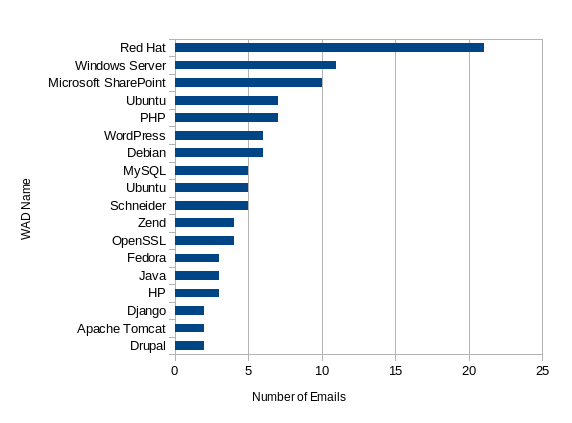
\includegraphics[width=1.0\textwidth]{emails_per_wad}
  \caption{Number of Email Alerts Sent for Each WAD Name in a Two-month Simulation}
  \label{figure:emails_per_wad}
\end{figure}

\paragraph{Accuracy}
Now we are going to have a closer look at the critical vulnerabilities that affected CERN (the green cells from table \ref{table:vnt_results}) to evaluate the tool and we will go over some statistical data obtained from the tool.
Figure \ref{figure:emails_per_wad} shows the number of emails that would be sent per each WAD name. This chart contains only the WAD names that occur more than once. From this figure one can get an idea of the most vulnerable technologies used at CERN. But we should keep in mind that the accuracy of our name matching algorithm has a direct impact on the number of emails we send for each WAD name. For example, if we look at all the vulnerabilities that have been matched to the WAD name `Red Hat', we realize that among the 21 emails that are sent, only 12 of them are in fact referring to the Red Hat operating system and the  other 9 are a consequence of false positives in our matching algorithm. Figure \ref{figure:emails_per_wad_fp} shows the number of true positive and false positive emails per WAD name and can be a better indicator of the most vulnerable products at CERN. For example, although more emails were sent about Debian, it does not mean that Debian has been more vulnerable than OpenSSL.
\\
\begin{figure}[H]
  \centering
    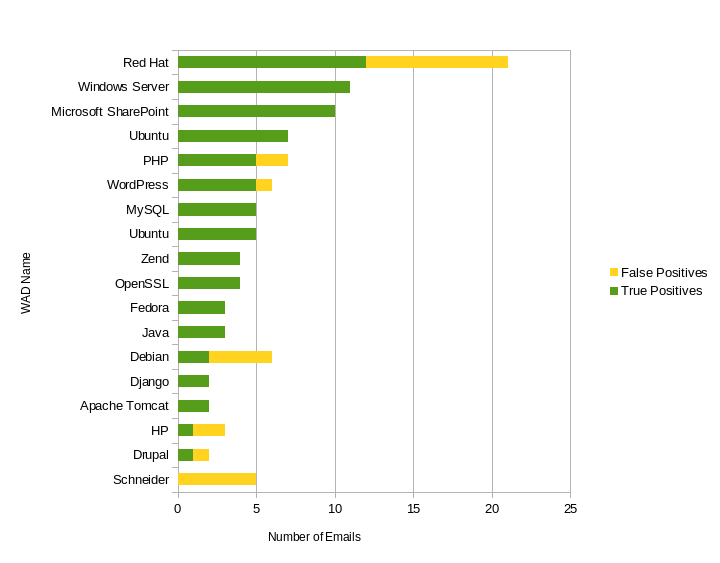
\includegraphics[width=1.0\textwidth]{emails_per_wad_fp}
  \caption{Number of Email Alerts Sent for each WAD Name in a Two-month Simulation}
  \label{figure:emails_per_wad_fp}

\end{figure}



\paragraph{Name Matching Accuracy}
Figure \ref{figure:fp_rate} shows that in 23\% of the cases the matching from the CPE to a WAD name has been wrong (too generic WAD names like `Red Hat'). The accuracy of the matches has been checked manually to get the data for this chart.

\begin{figure}[H]
  \centering
    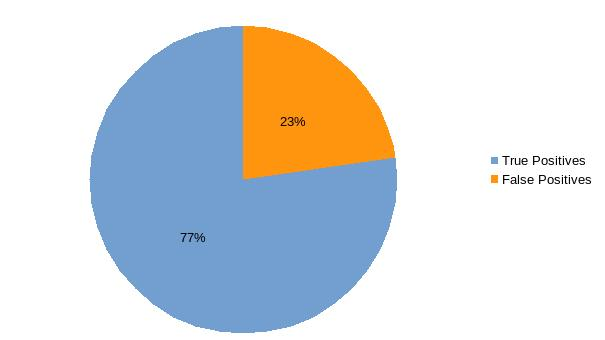
\includegraphics[width=1.0\textwidth]{fp_rate}
  \caption{False Positive Rate in Name Matching}
  \label{figure:fp_rate}

\end{figure}


\paragraph{}
Table \ref{table:vnt_results} shows that in 90\%  of the cases the email contains updated vulnerability information. Looking at the updated fields, we can see that most of the times the affected products (CPEs) are the fields that change. Figure \ref{figure:updates} shows the frequency of changes in different fields. Further investigation shows that the CVSS Score field has always changed from ``None" (no information available) to a value. This is expected as it usually takes some time (one or two days) until a CVSS score is available and once it is available it is highly reliable and it does not change. This does not hold for CPE name changes and in 20\% of the cases the CPE field changes from a non empty value.




\begin{figure}[h!]
  \centering
    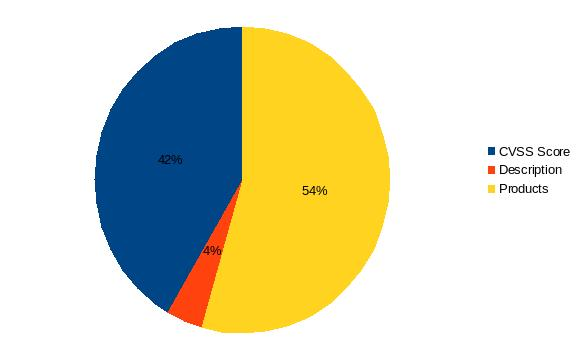
\includegraphics[width=1.0\textwidth]{updates}
  \caption{Updated Fields in Vulnerabilities}
  \label{figure:updates}

\end{figure}

















\chapter{Scanner}
\label{scanner}
\thispagestyle{empty}

\section{Motivation}
\label{scanner_motivation}
Chapter \ref{vulnerability-notification-tool} introduced the Vulnerability Notification Tool that is designed to identify CERN resources that might be affected by vulnerabilities associated with specific software components, however, sometimes we are not able to accurately detect software components on CERN resources (due to WAD limitations) or some vulnerabilities are not specific to any component and spotting them takes targeted scanning, which is the topic of this chapter. 
\paragraph{}
The CERN Computer Security Team performs scans of various types of resources, such as devices, web servers, web sites, etc. It is impossible to scan these resources manually and there is a need for a scanning engine to facilitate scheduling and running these scans, share the load across multiple scanning hosts in a fault-tolerant way, and combine the results.
\paragraph{}
``GNU Parallel" is a command-line utility for Unix-like operating systems that allows executing jobs concurrently locally or on remote computers. A job is typically a single command or a small script that has to be run for each of the lines in the input\footnote{\url{http://savannah.gnu.org/projects/parallel}}. It is trivial to provide GNU Parallel with a list of CERN resources and have the scans run on these resources concurrently.
\paragraph{}
On the other hand, as discussed in Section \ref{sec:tools}, CERN has a collection of scripts for detecting misconfigurations, such as expired certificates and basic HTTP authentication, or vulnerabilities, such as Heartbleed. 
\paragraph{}
There is a need for a tool that fills the gap between detection scripts and GNU Parallel to enable the continuous and automatic scanning of resources. This tool (the Scanner) is meant to act like as a wrapper around detection scripts, standardizing the input and output format of the scripts, so that parallel runs of it can be triggered by GNU Parallel and their results can be analyzed automatically. The Scanner should also make it possible to run a subset of available detection scripts on targets. Another objective of the Scanner is to make it as simple and fast as possible to add a new detection
\begin{figure}[H]

  \centering
    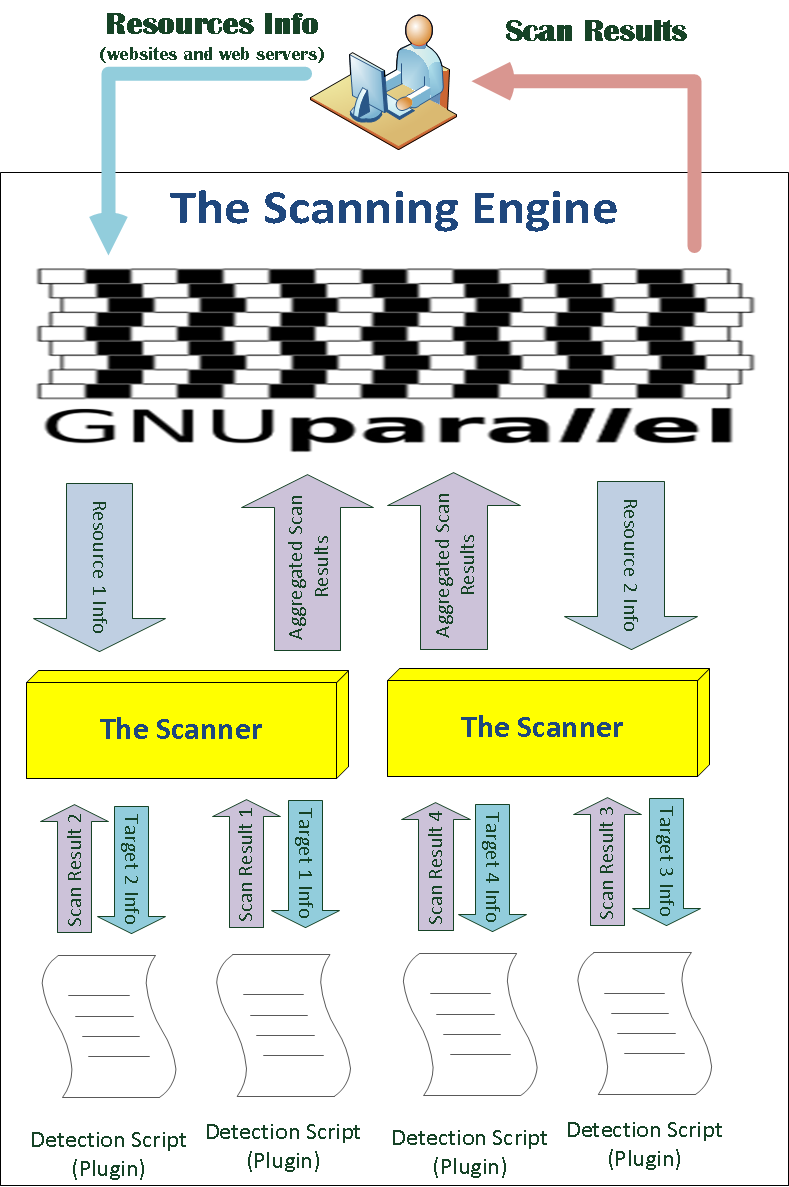
\includegraphics[width=1.0\textwidth]{scanner-architecture}
  \caption{Scanning Engine Architecture}
\label{figure:scanner-arch}
\end{figure}
\noindent
script, and run it on all CERN resources to ensure an acceptable detection/response speed when new vulnerabilities emerge. Figure \ref{figure:scanner-arch} illustrates the relation between the detection scripts, the Scanner and GNU Parallel. 




%TODO: include the diagram here
\subsection{Use Cases}
There are two major use cases for the Scanner:
\begin{itemize}
\item \textbf{Manual execution}: When we need to run an existing set of detection scripts on a new target (or existing targets, to get fresh results), or when we need to create a new script (e.g. Heartbleed test, when OpenSSL vulnerability surfaced) on the usual targets.
\item \textbf{Automatic execution}: For continuous scanning of stable target lists (e.g. all official web sites, all web servers exposed on the firewall, etc.) with relevant test sets.
\end{itemize}

\section{Scanner Specifications}
The Scanner runs a set of security tests (called plugins) on a single resource, and collects, combines and delivers plugins scan results. When calling the Scanner, we ask it to scan a given resource type with a unique name. The Scanner ensures that only plugins for that resource type will be executed. 

\subsection{Plugin Specifications}
A plugin is a single security test for a given type of resource. After scanning a target, it says if a security problem was found or not (it can output more details when relevant). Detection scripts described in section \ref{sec:tools} are examples of plugins.
%delam gerefte ey doost, havaye gerye ba man...havaye gerye ba man...
\subsubsection{Resource Types}
There are various types of resources at CERN. In most cases the plugins need to scan websites or web servers (or other devices), but our implementation of the Scanner is independent of the type of the resource that is being scanned. If a plugin scans more than one resource type, depending on the type of the resource, it will require different inputs and consequently it needs to be executed differently. The Scanner, on the other hand, is the tool that executes the plugins. Therefore, it needs to be configured to execute the same plugin in different ways depending on the resource type. To avoid complexity or ambiguity, a given plugin should deal with only one type of resource. Occasionally, the same test will need to be developed for different types of resources (e.g. the default landing page test is needed for both web sites and web servers). In that case, the logic of the test should be shared, but still separate scripts should be developed for each resource type. For example, imagine that the script \texttt{landing\_page.py} contains the logic for testing for a default landing page on websites and web servers. A possible implementation is to develop one script for websites (\texttt{landing\_page\_site.sh}) that runs `\texttt{./landing\_page.py -site \$1}' and one script for web servers (\texttt{landing\_page\_server.sh}) that runs `\texttt{./landing\_page.py -server \$1}' 
\subsubsection{Input}
The Scanner provides the plugin with inputs it should process. Depending on the nature of the security test a plugin is performing, it needs different input data. It is important that all plugins follow a convention about the way they receive inputs, so that the Scanner can run all the plugins in the same way. A plugin can assume that it is going to receive the input in the following order: \{\texttt{IP/HostName PORT ALIAS URL}\} for web servers/devices and \{\texttt{URL}\} for websites. The plugin can decide to ignore any of these input arguments, if irrelevant. Also, the Scanner might pass an empty string if the user does not specify a field.
Additionally, plugins can be called with the following arguments instead of the target resource:
\texttt{-{}-info} - returns plugin details in JSON format (see Figure \ref{figure:plugin-info})  
\begin{figure}[h!]

  \centering
    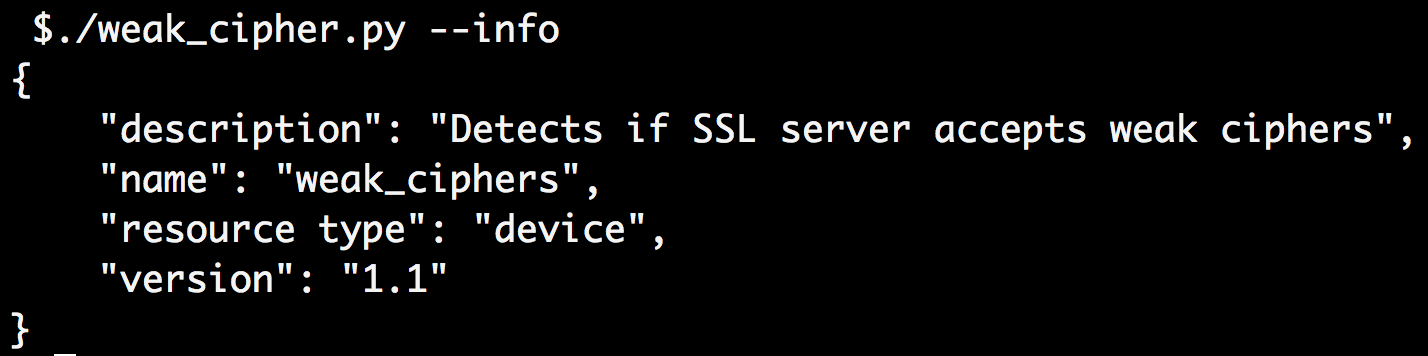
\includegraphics[width=1.0\textwidth]{plugin-info}
  \caption{Plugin Information}
\label{figure:plugin-info}
  
\end{figure}
\subsubsection{Output}
It is important that the plugins follow a convention in their output format, so that the Scanner can analyze the results and group them, if necessary. Figure \ref{figure:plugin-results} illustrates a sample plugin output. After scanning a given target, each plugin should return the following information in JSON format (mandatory fields in bold): 
\begin{itemize}


   \item \textbf{result} (mandatory): severity of the findings; one of these values (any other value in the result will be accepted by the Scanner, but a warning will be logged):
    \begin{itemize}
    

        \item \textit{SECURE} - no security problem was found.
        \item  \textit{VULNERABLE} - security problem detected.
        \item  \textit{WARNING} - there is something sub-optimal (e.g. a certificate expiring soon) but not a real security problem, yet.
        \item  \textit{TIMEOUT} - results not available, test timed out (the plugins do not have to recover from timeouts as this can be done in the Scanner level).
        \item  \textit{UNKNOWN} - results not available, test couldn't conclude (e.g. host unreachable).
      
            \end{itemize}
\item      \textbf{notes} (mandatory): human-readable details of the scan result (e.g. which weak ciphers were detected, which URLs are affected).
\item      target (recommended): what was scanned: If the target information is provided by the plugin it can be used to show more precise results, for example if a default port has been used, etc. The plugin can choose to report all or a subset of following:
\begin{itemize}


\item        host
\item    port
\item    alias
\item    url 
\end{itemize}
\item    plugin info (recommended):
\begin{itemize}
\item        name
\item        version
\item    resource type
\item    description - a one-line description of the plugin. 
\end{itemize}
\end{itemize}



\begin{figure}[h!]
  \centering
    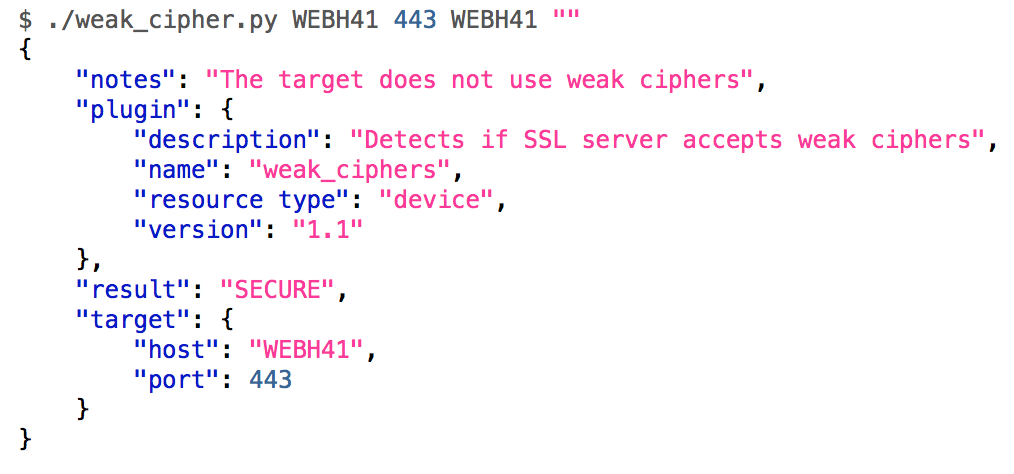
\includegraphics[width=1.0\textwidth]{plugin-results}
  \caption{Plugin Output}
  \label{figure:plugin-results}
  
\end{figure}



\subsection{Scanner Options}
The Scanner will be directly used by the CERN Security Team members; therefore, it is important to design a robust user interface for it. The user can use the following options to customize Scanner parameters:

\begin{itemize}

\item 

    \texttt{-l|-{}-list TYPE} - list all plugins available in the plugin directory 
                       (for the given resource type(or all)).
\item    \texttt{-q|-{}-quiet} - be quiet (only output the scan result and no other information regarding the progress of the scan).
\item    \texttt{    -v|-{}-verbose LEVEL} - be more verbose. 
    	 				 (to the given verbosity level in the range of 1 to 5,
    	 				  with 5 being the most verbose).
\item    \texttt{    -t|-{}-timeout SECONDS} - set timeout per plugin (same for all plugins).
\item    \texttt{    --plugin PLUGIN1.sh,PLUGIN2.py,PLUGIN3} - run selected plugins.
\item    \texttt{ -{}-plugin-list PLUGINS-FILE} - run plugins listed in the file (one line per plugin executable).
\item    \texttt{  -{}-plugin-dir DIRECTORY} - look for plugins in this directory. %TODO: check with Sebastian (default: /opt/scan/plugins)
\item    \texttt{    -{}-log FILE} - log output (but not results) to a file instead on printing on standard output.  
\end{itemize}
\clearpage
And the following options can be used to define the target resource:
\begin{itemize}

    \item    \texttt{-{}-device NAME} - scan the device (mandatory for devices).
    \item    \texttt{-{}-website NAME} - scan the centrally hosted website (mandatory for websites).
%    \item    \texttt{-{}-account NAME} - scan the account (mandatory for accounts)
%    \item    \texttt{-{}-set NAME} - scan the set (mandatory for sets)
    \item    \texttt{-{}-ip IPs} - set device target IP addresses (comma separated values).
    \item    \texttt{-{}-port PORTs} - set device target port numbers (comma separated values).
    \item    \texttt{-{}-alias ALIASes} - set device target aliases (comma separated values).
    \item    \texttt{-{}-url URLs} - set device/website target URLs (comma separated values). For devices a url means more like a directory on the device. 
   \end{itemize}
   


\subsection{Targets}
A CERN resource can be composed of multiple targets. For example, a device can have multiple IP addresses, aliases, open ports or URLs and each combination of these fields can specify a scanning target. A plugin deals with only one target (a single IP, alias, port, etc.) and it is the job of the Scanner to loop over all combinations of IP addresses, aliases, ports and URLs when calling plugins .
\subsubsection{Example}
Consider the following command:

\begin{table}[H]
\begin{center}
    \begin{tabular}{ c  l }


\$ \texttt{./scanner.py} &  \texttt{-{}-plugin basic\_auth.py}  \\
			   &  \texttt{-{}-device PCITDI86}  \\
			   &  \texttt{-{}-ip 137.138.43.51,2001:1458::112:33} \\
	           &  \texttt{-{}-port 80,443  }\\
	           &   \texttt{-{}-alias CSC,PHOTOCLUB}  \\
    	       &  \texttt{-{}-url /admin,/tmp}
    	       
	\end{tabular}
    
   \end{center}
\end{table}
\noindent
With this command the Scanner will run the Basic Authentication plugin (which checks if the target is doing the authentication over HTTP instead of HTTPS) on a resource of type `device' and with the name `PCITDI86'. In addition, there are multiple IP addresses, aliases, ports and URLs that we would like to scan. The Scanner is going to run the plugin 2*3*2*2=24 times on PCITDI86. Table \ref{table:targets} shows the different targets that will be scanned. 

\begin{table}
\begin{center}
    \begin{tabular}{ | c | c | c | c |}
    
    \hline
	  \hhline{|*4-}
  \multicolumn{1}{|c|}{\cellcolor{LightBlue}\textbf{IP/Hostname}} & \multicolumn{1}{|c|}{\cellcolor{LightBlue}\textbf{Port}} 
  & \multicolumn{1}{|c|}{\cellcolor{LightBlue}\textbf{Alias}} &    \multicolumn{1}{|c|}{\cellcolor{LightBlue}\textbf{URL}}    
    \\ \hline

   \multirow{12}{*}{137.138.43.51} &     \multirow{6}{*}{80} &     \multirow{2}{*}{PCITDI86} & /admin
   \\
    \cline{4-4}
       &     &     & /tmp
    \\
     \cline{3-4}
	& & \multirow{2}{*}{CSC} & /admin
	\\
	 \cline{4-4}
       &     &     & /tmp
    \\
     \cline{3-4}
 	& & \multirow{2}{*}{PHOTOCLUB} & /admin
	\\
	 \cline{4-4}
       &     &     & /tmp
    \\
     \cline{2-4}
    
    & \multirow{6}{*}{443} &     \multirow{2}{*}{PCITDI86} & /admin
   \\
    \cline{4-4}
       &     &     & /tmp
    \\
     \cline{3-4}
	& & \multirow{2}{*}{CSC} & /admin
	\\
	 \cline{4-4}
       &     &     & /tmp
    \\
     \cline{3-4}
 	& & \multirow{2}{*}{PHOTOCLUB} & /admin
	\\
	 \cline{4-4}
       &     &     & /tmp
    \\
     \cline{1-4}
     
     
     
     
     
     \multirow{12}{*}{2001:1458::112:33} &     \multirow{6}{*}{80} &     \multirow{2}{*}{PCITDI86} & /admin
   \\
    \cline{4-4}
       &     &     & /tmp
    \\
     \cline{3-4}
	& & \multirow{2}{*}{CSC} & /admin
	\\
	 \cline{4-4}
       &     &     & /tmp
    \\
     \cline{3-4}
 	& & \multirow{2}{*}{PHOTOCLUB} & /admin
	\\
	 \cline{4-4}
       &     &     & /tmp
    \\
     \cline{2-4}
    
    & \multirow{6}{*}{443} &     \multirow{2}{*}{PCITDI86} & /admin
   \\
    \cline{4-4}
       &     &     & /tmp
    \\
     \cline{3-4}
	& & \multirow{2}{*}{CSC} & /admin
	\\
	 \cline{4-4}
       &     &     & /tmp
    \\
     \cline{3-4}
 	& & \multirow{2}{*}{PHOTOCLUB} & /admin
	\\
	 \cline{4-4}
       &     &     & /tmp

	
        \\ \hline
    \end{tabular}
    \caption{Targets}
    \label{table:targets}
   \end{center}
\end{table}

For many plugins (e.g. Heartbleed) the URLs are irrelevant, while for others (e.g. basic\_authentication) the possibility to scan several URLs/sub-directories for a given host name is very useful. Obviously, we want to avoid that the Scanner loops over multiple URLs when scanning for Heartbleed. This means that some plugins (e.g. Heartbleed and basic-authentication) should not be used together for the same target details, but rather separately: 

\begin{table}[H]
    \begin{tabular}{ c  l }


\$ \texttt{./scanner.py} & \texttt{-{}-plugin-list https-plugins.txt} \\
  & \texttt{-{}-device PCITDI86} \\
  & \texttt{-{}-alias CSC,PHOTOCLUB}\\
  & \texttt{-{}-port 443,8123}\\
  \\
  
    	       \$ \texttt{./scanner.py} & \texttt{-{}-plugin basic-auth.py} \\
  & \texttt{-{}-device PCITDI86} \\
  & \texttt{-{}-alias CSC,PHOTOCLUB}\\
  & \texttt{-{}-port 80,443,8123}\\
    	       & \texttt{-{}-url /admin,/tmp}
    	       
	\end{tabular}
    
\end{table}
\noindent
If, incidentally or pressed by an emergency, we call the Scanner and provide ``too many" details for plugins that do not need them, things should still work. We just risk waiting for the results a bit longer, and getting duplicated results.
\subsection{Output}
The Scanner prints exactly one line per resource and vulnerability, in the form of semicolon-separated values:
\begin{verbatim}
resource_type;resource_name;plugin_name;result;notes;targets
\end{verbatim}
Targets from the same resource with the same scanning results (including the notes) will be grouped into one line. This gives the plugin designer the opportunity to decide on grouping. For example, if the plugin designer includes the port number in the notes, the targets with the same results but different port numbers will be reported in two different lines. This is useful, because the grouping very much depends on the nature of the test the plugin is running. For example, in the case of Heartbleed, the plugin designer would prefer to include the IP address and port number in the notes, but ignore the URLs. On the other hand, the landing\_page plugin needs to report the complete target fields, including URLs, in the notes.
\subsubsection{Examples}
The following command checks if the device uses SSL3\footnote{SSL version 3 is vulnerable to the POODLE vulnerability discovered in October 2014}:
\begin{table}[H]

    \begin{tabular}{ c  l }


\$ \texttt{./scanner.py} & \texttt{-{}-plugin detect\_ssl3.py } \\
  & \texttt{-{}-device PCITDI86} \\
  & \texttt{-{}-port 443,8443}    	       
	\end{tabular}    

\end{table}
\noindent
The output of the scan is: 
\\
\\
\texttt{
\#resource\_type;resource\_name;test\_name;result;notes;target}
\\
\\
\texttt{device;PCITDI86;detect\_ssl3;VULNERABLE;SSLv3 is enabled on PCITDI86:443;[PCITDI86:443]}
\\
\\
\texttt{device;PCITDI86;detect\_ssl3;VULNERABLE;SSLv3 is enabled on PCITDI86:8443;[PCITDI86:8443]}
\\
\\
As one can see, for each scan a different result line is printed, because the plugin reports the device name and port in the notes. 
This other example checks for a default landing page on a web server:
\begin{table}[H]

    \begin{tabular}{ c  l }


\$ \texttt{./scanner.py} & \texttt{-{}-plugin landing\_page.py } \\
  & \texttt{-{}-device pcitdi86} \\
  & \texttt{-{}-alias pcitdi86-alias}\\    	       
    & \texttt{-{}-url /index.html}\\ 
	\end{tabular}    

\end{table}
\noindent
The output will be:
\\
\\
\texttt{
\#resource\_type;resource\_name;test\_name;result;notes;targets}
\\
\\
\texttt{
device;pcitdi86;landing\_page;SECURE;The target does not use an empty or default page;[pcitdi86-alias(pcitdi86):80/index.html,pcitdi86:80/index.html]
}
\\
In this case, the scanning results of the two targets (with different aliases) are grouped into one line.
If the Scanner faces a problem while running the plugin (plugin crash, output not parsable, etc) it will report a line with the result FAIL. Also, if the user defines a timeout (via -{}-timeout) and a timeout occurs while running the plugin, it will be reported in the final results.
\\ 
\texttt{device;pcitdi87;landing\_page;TIMEOUT;plugin timeout after 10 ms;[pcitdi86:80/index.html]}
\\
\\
\texttt{device;pcitdi88;landing\_page;FAIL;There was a problem parsing plugin output(error code 127);[pcitdi86:80/index.html]}
\\
\\
%\section{Implementation}
%\subsection{Directory Structure}
%The plugins directory can be set by using the option -{}-plugin-dir. Each plugin should be placed in its corresponding resource type directory. Therefore, the plugins directory contains the following sub-directories:
%\begin{itemize}
%
%
%   \item \texttt{/device}
%    \item \texttt{/web}
%    \item \texttt{/account}
%    \item \texttt{/site} 
%    
%    \end{itemize}
%
%note that all executable files in these directories are considered plugins. In particular, they all will be executed(!), when we call \texttt{./scanner.py -{}-list TYPE}

\section{Conclusion}
The Scanner fills the gap between a scanning engine and individual security tests. It makes it easier to develop detection scripts that would test for a misconfiguration or a vulnerability on a single target. This can improve the procedure of scanning CERN resources, whenever a new vulnerability is discovered. Using the Scanner we can develop short detection scripts that deal with only one target and use the Scanner to take care of looping over different targets on the same resource. One level higher, we would like to scan multiple resources at CERN (maybe the whole CERN infrastructure) to find vulnerable resources, in a concurrent and fault tolerant manner. GNU Parallel as described in Section \ref{scanner_motivation} can feed the resource data (from prepared files, obtained by running \texttt{was list-servers} and \texttt{was list-sites}) to the Scanner and have it scan multiple resources concurrently.
\paragraph{}
In addition, the Scanner will group the findings of individual tests to remove duplicate results and generate a parsable output that can be used for further investigations. For example, the Scanner output can be inserted into the CERN System Security DataBase (SSDB), used to keep track of vulnerabilities. Integration to SSDB is not implemented, yet, because SSDB will soon be replaced by an improved solution. 


\chapter{Conclusion and Future Work}
\label{conclusion-and-future-work}
This project introduced two new tools for detection of vulnerable web applications deployed in a large IT installation. The approaches used in these tools are different from common web scanners, such as Skipfish. In this project we focused more on detecting vulnerable applications as soon as possible by monitoring publicly available vulnerability information. Once we are aware of a vulnerability, we can take two approaches to detect applications that may be a subject to it. If the vulnerability is specific to a software or product, VNT described in Chapter \ref{vulnerability-notification-tool} will report the resources (applications) that use those products. In other cases when the vulnerability is not specific to one product but to its configurations, e.g. an expired certificate, or when detecting the vulnerable technology on resources or applications is not possible or efficient, e.g detecting technologies not supported by WAD, the Scanner (Chapter \ref{scanner}) can be used to run other detection scripts. In addition, the Scanner can be used to run automated regular scans of the whole web infrastructure at CERN and analyze the scan results automatically. Both of these tools are currently being used at CERN to enhance the vulnerability management process of web applications, but there is a potential for improvements in both of them. 
 
\section{Vulnerability Notification Tool}
VNT can be used to get informed about all vulnerabilities, regardless of the product they affect or whether they are web-related. At the moment, it stores all these findings in parsable files. Therefore, it can become a part of the overall CERN vulnerability management mechanism to help keep track of vulnerabilities anywhere. It is possible to extend VNT and evolve it into a vulnerability management framework, where users can decide to ignore some vulnerabilities or get different notifications based on the type of the changes that happen in a vulnerability.
\paragraph{}
The performance of VNT is highly dependent on the vulnerability source it is using. At the time of this project, it was decided to use NVD,  but it is important to keep an eye on the market and use other sources instead of --or along with-- NVD, if they fit the needs described in Section \ref{source_evaluation}. 

\paragraph{}
One of the main challenges while using NVD as the vulnerability source, was the randomness of CPE names. Although CPE is introduced as a standard way of enumerating platforms, there are still many problems with it: Its dictionary is incomplete and contains redundant entries, such as multiple CPE names for the same product. On the other hand, it seems that the available vulnerability sources have not agreed on a standard way of listing vulnerable softwares and each has come up with its own format. The CPE name mapping algorithm described in Section \ref{name_matching} has been tested on NVD CPE data, but would probably be efficient enough on other naming formats with some minor changes. In any case, there seems to be a need for a standard product naming format that is complete and robust enough to meet the requirements of all interested parties. 

\paragraph{}
The product name matching algorithm that is currently being used to find vulnerable products can also be improved. In addition to application names, WAD provides the category (type) of each application. The current algorithm described in Section \ref{name_matching} ignores the category of WAD names. A possible improvement to the algorithm would be to report matches only if the CPE type (first field of the CPE name) and WAD category match (e.g. both are operating systems). Another potential improvement is to use available algorithms for computing the string distance between CPE and WAD names, reporting only the pairs that have a similarity higher than a decided threshold.  

\paragraph{}
Alternatively, WAD can be extended to include the equivalent CPE name(s) for each WAD name. This approach can ensure a higher accuracy level, because there will be no need for a name matching algorithm. However, maintaining this dictionary of WAD names to CPE names will be necessary whenever new WAD names are added to WAD. Ideally, this extension can be done to Wappalyzer to benefit from the community of Wappalyzer to maintain the dictionary. But Wappalyzer does not have a security purpose and it would be a challenge to convince its community to care for finding equivalent CPE names whenever they add a new detection rule for a new technology. 

\paragraph{}
NVD reports a list of affected product versions, but this data changes very often. One can notice that previously announced vulnerable versions sometimes get removed from NVD updates or versions that were not reported as vulnerable, enter the list. There are many cases where vulnerability information gets updated on NVD with a small change in the sub-sub-version of an affected product. If VNT was sending update notifications for every change in affected product versions, it would flood its users with updates, encouraging them to ignore such notifications completely. Therefore, in the current tool, we decided to ignore any changes in product versions. Apparently, knowing about these changes can be useful in some cases though. Imagine that there is a vulnerability that is affecting Drupal version 6. We might decide to ignore this vulnerability at CERN, because all Drupal instances are using version 7 or higher. If a couple of days later, NVD updates the same vulnerability and lists Drupal 7 as a vulnerable product, we would definitely like to receive an update notification. As one can see, there is a trade-off here and it can be an open question to the CERN Computer Security Team to decide if they would rather receive more notifications (among which many are useless), for the sake of not missing important product version changes in vulnerability information.
\paragraph{}
For the time being, VNT is sending email notifications to the CERN Computer Security Team members rather than the resource owners. The reason is that, in most cases, further investigation of a vulnerability is needed to make sure that the reported resources are indeed affected. One step towards fully automating the tool is to consider product versions when reporting the resources.
\paragraph{}
The product version reported by WAD, however, is not always reliable. For instance, Apache servers might be reported to have obsolete versions while the new updates have been back-ported\footnote{Parts of a newer version of a software have been added to an older version of the same software, without upgrading.} to them. In addition, WAD is unable to detect the version of many products, e.g. CakePHP framework. Due to these limitations, it was decided to ignore product versions when reporting vulnerable resources and leave it to the investigator of the vulnerability to decide if a certain resource is indeed affected. Once WAD supports more reliable version detection, VNT can be slightly changed to only report resources that use a certain version of a product.
\paragraph{}
Used in a slightly different way, VNT can be used to make sure that new resources at CERN are not vulnerable. Whenever there is a new resource detected by WAD, we can use VNT data to ensure that this new resource is not vulnerable to recently found vulnerabilities.
\section{Scanner}
The Scanner facilitates running individual detection scripts on CERN resources. Currently, it supports detection scripts that run on websites and web servers (devices). It can be easily extended to support other types of resources at CERN. For example, CERN is managing user accounts and each of these accounts can be considered as a resource. Each account is associated with an AFS space and one can think of scanning all accounts at CERN to find out if a user is storing his private keys in an AFS public folder. This would be a security risk for the user, because everyone in the organization would have access to his private key. The Scanner could be used to run this script on all accounts at CERN if provided with relevant inputs to pass into the detection script.
%% change the example: for example talk about checking public / private key available on AFS
%a password has been exposed (when a list of exposed email addresses and passwords is advertised publicly) and write a detection script for this purpose. 
\paragraph{}
Currently VNT and the Scanner are two separate tools for different purposes. In cases that a vulnerability detected by VNT needs further investigations, it would be valuable to connect VNT to the Scanner. This could help the CERN Computer Security Team test for themselves whether a given server or site is actually subject to a VNT-reported vulnerability by writing a corresponding plugin and launching the Scanner to check the VNT-reported targets, then automatically trigger a mail notification if the vulnerability is confirmed.


\bibliographystyle{unsrt}
\addcontentsline{toc}{chapter}{Bibliography}

\nocite{*}

\thispagestyle{empty}
\bibliography{bibliography}
\begin{appendix}
\appendix
\chapter{VNT Evaluation Method}
\label{vnt_evaluation_method}
Once we have the output of the tool in JSON format, it is easy to convert it to other formats to do an analysis of the results or obtain some statistics. 
\subsection{Calculating the Number of Vulnerabilities}
The python script \texttt{vnt\_format.py} receives the JSON description of VNT results as an input and generates an output in text format describing each vulnerability in one line. This text output can be used by various command line tools, such as grep, cut, etc., to obtain statistics. 
Each line is in the following format:
\begin{framed}

\texttt{c|n;%published\_date;last\_modified\_date;reported\_date;cve\_id;nvd\_description\_url;
cvss\_score;%cpe\_names;
wad\_names
%;
%changed\_field\%old\_value\%new\_value
}

\end{framed}
The first component describes if the vulnerability is new (n) or has changed (c). If there are multiple entries in one component, i.e multiple WAD names, entries are separated by comma.
\\
For Example:
\begin{framed}
\texttt{c;6.8;Red Hat,Fedora,JBoss Web,OpenSSL}
\end{framed}
describes a vulnerability that has changed, has a CVSS score of 6.8 and matches with WAD names `Red Hat', `Fedora', `JBoss Web' and `OpenSSL'.
The following command will output the number of new vulnerabilities and changes in vulnerabilities using the TEXT description of all the results. 
\begin{framed}
\begin{verbatim}
$ cat *.txt| cut `-d;' -f1| sort| uniq -c
\end{verbatim}
\end{framed}
In order to get the critical vulnerabilities one can use the following command:
\begin{framed}
\begin{verbatim}
$ cat *.txt| grep `;\([6-9]\|10\)\.'| cut `-d;' -f1| sort|\
  uniq -c
\end{verbatim}
\end{framed}
It is also important to know the number of vulnerabilities that affect CERN. For this purpose WAD can be used to generate a file with all WAD names used at CERN (one name per line) and then using the following command can give us the same statistics as before, but only considering the vulnerabilities that affect CERN.
\begin{framed}
\begin{verbatim}
$ cat *.txt| grep -f wad_names_at_cern.txt| cut `-d;' -f1|\
  sort| uniq -c
\end{verbatim}
\end{framed}
\begin{framed}
\begin{verbatim}
$ cat *.txt| grep -f wad_names_at_cern.txt|\
  grep `;\([6-9]\|10\)\.'| cut `-d;' -f1| sort|\
  uniq -c
\end{verbatim}
\end{framed}
%
%
\chapter{Implementation Details}
\label{implementation-details}
\section{Vulnerability Notification Tool}

Figure \ref{figure:vnt-internal-arch} illustrates the internal architecture of VNT. 
As you can see there are 2 classes and four scripts in the tool. Class Vulnerability represents vulnerabilities with all their NVD reported fields. 
Class Product takes care of everything that is related to CPE names. The main method in this class is the \texttt{guess\_wad\_names()} method which implements the mapping algorithm. 
Different mapping algorithms were tested and all of them are implemented in this class, however the best one was chosen to be called when mapping was necessary. \texttt{vnt-init.sh} is a shell script that can be used to initialize the tool when it is being deployed on a new machine. This script downloads yearly feeds from NVD and stores all the vulnerability data, so that in future executions, the tool can discover new or updated vulnerabilities. \texttt{send-notification.sh} is the main script of the tool, in the sense that it uses both main components of VNT (VNT\_CORE and VNT\_EMAIL) to download the feeds and report vulnerabilities.
\paragraph{}
VNT needs to have WAD names (apps.txt) to match CPE names to WAD names and WAD findings at CERN (wad_finidings_cern.txt) to filter out the irrelevant vulnerabilities. These two text files were generated using WAD. 
\begin{figure}[h!]
  \centering
    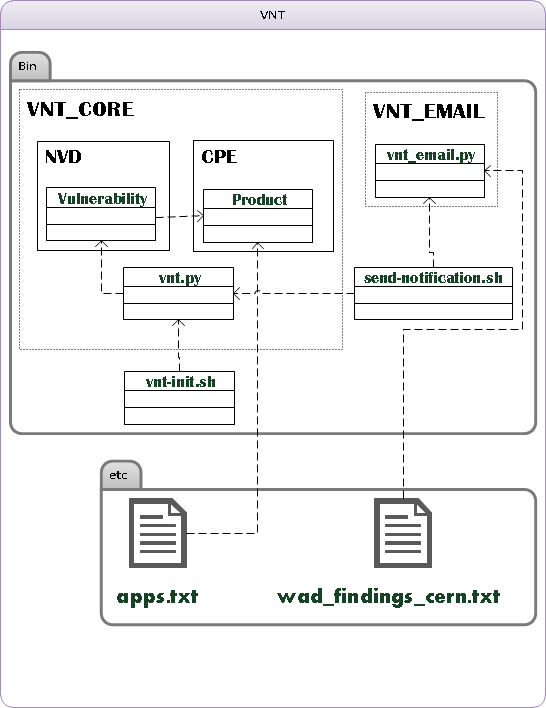
\includegraphics[width=1.0\textwidth]{vnt-internal-arch}
  \caption{VNT Internal Architecture}
   \label{figure:vnt-internal-arch}
\end{figure}

\paragraph{}
Python 2.6 was used as the main programming language for this project (except for the shell scripts) and a total of 1,026 lines of code were developed for this tool. 
\section{Scanner}
Figure \ref{figure:scanner-internal-arch} illustrates the internal architecture of the Scanner. The Scanner is using 4 main Python classes to represent targets, plugins, plugin output and scan results. \texttt{scanner.py} is the main script of the tool to execute when scanning targets. The Scanner is dependent on the available plugins. In order to be able to test the Scanner, it was necessary to develop some plugins or modify the existing ones to follow the Scanner conventions. For this purpose the plugin \texttt{landing\_page.py} for both websites and servers were developed.
\begin{figure}[h!]
  \centering
    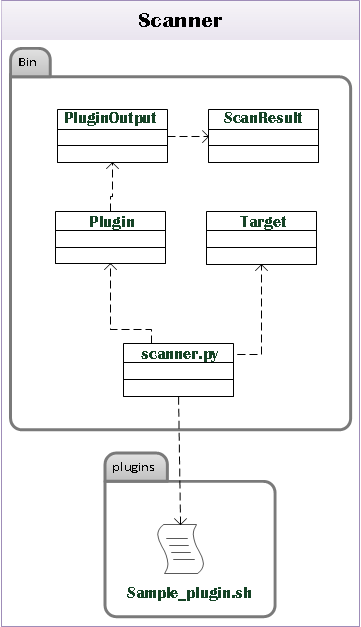
\includegraphics[width=1.0\textwidth]{scanner-internal-arch}
  \caption{Scanner Internal Architecture}
   \label{figure:scanner-internal-arch}
\end{figure}
\end{appendix}
\end{document}






